\documentclass[11pt,a4paper]{ctexart}
\usepackage{../../../common/ipara}
\usepackage{tikz-3dplot}
\usetikzlibrary{calc}
\raggedbottom

% =====================================================
% 题型：立体几何解答题 / 折叠与最值问题 (q_solid_folding_rectangle.tex)
% =====================================================
% =====================================================
% 难度：★★★ (难题)
% =====================================================
\newcommand{\qSolidFoldingRectangleStem}{%
  如图，在矩形 $ABCD$ 中，$AB=1$，$BC=\sqrt{3}$，$M$ 是线段 $AD$ 上的一动点，将 $\triangle ABM$ 沿着 $BM$ 折起，使点 $A$ 到达点 $A'$ 的位置，满足点 $A' \notin$ 平面 $BCDM$，且点 $A'$ 在平面 $BCDM$ 内的射影 $E$ 落在线段 $BC$ 上。
  \begin{enumerate}[label=(\arabic*), leftmargin=2em, itemsep=0.1em]
    \item 当点 $M$ 与端点 $D$ 重合时，证明：$A'B \perp$ 平面 $A'CD$；
    \item 当 $AM=\dfrac{3}{2}$ 时，求二面角 $A'-BM-C$ 的余弦值；
    \item 设直线 $CD$ 与平面 $A'BM$ 所成的角为 $\alpha$，二面角 $A'-BM-C$ 的平面角为 $\beta$，求 $\sin^2\alpha \cos\beta$ 的最大值。
  \end{enumerate}%
}

\newcommand{\qSolidFoldingRectangleFigure}[1][1.0]{%
  \begin{tikzpicture}[scale=#1, >=stealth, line join=round, line cap=round]
    % 左图：折叠前
    \begin{scope}[xshift=0cm, yshift=0cm]
      % 定义顶点
      \coordinate (B) at (0, 0);
      \coordinate (C) at (2.6, 0);
      \coordinate (D) at (2.6, 1.5);
      \coordinate (A) at (0, 1.5);
      \coordinate (M) at (1.8, 1.5);
      \coordinate (E) at (1.25, 0);
      \coordinate (F) at (0.74, 0.62);
      
      % 绘制矩形和折痕
      \draw[thick] (A) -- (B) -- (C) -- (D) -- cycle;
      \draw[thick, dashed, blue] (B) -- (M);
      \draw[thick, dashed, red] (A) -- (E);
      
      % 标记点
      \fill (A) circle (1.2pt) node[above left] {\small $A$};
      \fill (B) circle (1.2pt) node[below left] {\small $B$};
      \fill (C) circle (1.2pt) node[below right] {\small $C$};
      \fill (D) circle (1.2pt) node[above right] {\small $D$};
      \fill (M) circle (1.2pt) node[above] {\small $M$};
      \fill (E) circle (1.2pt) node[below] {\small $E$};
      \fill (F) circle (1.2pt) node[above left] {\small $F$};
      
      % 直角标记
      \draw[gray, thin] ($(F)!0.1!(A)$) -- ($($(F)!0.1!(A)$) + ($(F)!0.1!(M)$) - (F)$) -- ($(F)!0.1!(M)$);
      
      \node[below] at (1.3, -0.2) {\small 折叠前};
    \end{scope}
    
    % 折叠箭头
    \draw[->, very thick, gray] (3.0, 0.75) -- (4.0, 0.75) node[midway, above] {\small 折叠};
    
    % 右图：折叠后
    \begin{scope}[xshift=4.5cm, yshift=0cm]
      % 定义顶点 (精确计算的投影三维坐标)
      \coordinate (B) at (0, 0);
      \coordinate (C) at (2.6, 0);
      \coordinate (D) at (3.2, 0.9);
      \coordinate (M) at (2.55, 0.9);
      \coordinate (E) at (1.15, 0);
      \coordinate (A1) at (1.15, 0.96);
      \coordinate (F) at (1.02, 0.36); % BM 上的垂足 F
      
      % 绘制底面边界与棱
      \draw[thick] (B) -- (C) -- (D);
      \draw[thick, dashed, gray!60] (D) -- (M);
      \draw[thick, dashed, gray!60] (M) -- (B);
      
      % 绘制折起后的面 A'BM 和 A'BC
      \draw[thick, blue] (A1) -- (B);
      \draw[thick, blue] (A1) -- (M);
      \draw[thick] (A1) -- (C);
      \draw[thick, dashed, gray!60] (A1) -- (D);
      
      % 绘制辅助线
      \draw[thick, dashed, red] (A1) -- (E);
      \draw[thick, dashed, red] (E) -- (F);
      \draw[thick, dashed, red] (A1) -- (F);
      
      % 标记点
      \fill (B) circle (1.2pt) node[below left] {\small $B$};
      \fill (C) circle (1.2pt) node[below right] {\small $C$};
      \fill (D) circle (1.2pt) node[above right] {\small $D$};
      \fill (M) circle (1.2pt) node[above right] {\small $M$};
      \fill (E) circle (1.2pt) node[below] {\small $E$};
      \fill (A1) circle (1.2pt) node[above] {\small $A'$};
      \fill (F) circle (1.2pt) node[left] {\small $F$};
      
      % 直角标记
      % A'E \perp base
      \draw[red, thin] ($(E)!0.08!(A1)$) -- ($($(E)!0.08!(A1)$) + ($(E)!0.08!(B)$) - (E)$) -- ($(E)!0.08!(B)$);
      % A'F \perp BM
      \draw[red, thin] ($(F)!0.08!(A1)$) -- ($($(F)!0.08!(A1)$) + ($(F)!0.08!(M)$) - (F)$) -- ($(F)!0.08!(M)$);
      % EF \perp BM
      \draw[red, thin] ($(F)!0.08!(E)$) -- ($($(F)!0.08!(E)$) + ($(F)!0.08!(M)$) - (F)$) -- ($(F)!0.08!(M)$);
      
      \node[below] at (1.3, -0.2) {\small 折叠后};
    \end{scope}
  \end{tikzpicture}%
}

\newcommand{\qSolidFoldingRectangleAnswer}{%
  (1) 证明见解析；(2) 二面角 $A'-BM-C$ 的余弦值为 $\dfrac{4}{9}$；(3) $\sin^2\alpha \cos\beta$ 的最大值为 $\dfrac{1}{4}$.%
}

\newcommand{\qSolidFoldingRectangleSolution}{%
  【解题思路】\\
  本题为折叠几何综合最值难题。解题的关键在于抓住折叠前后的“距离与角度不变性”，通过代数建模构建起动态线段的长度关系网络：
  \begin{enumerate}[label=\arabic*.]
    \item \textbf{建立核心长度模型}：设 $AM=x$。通过 $A'$ 在底面的射影 $E$ 落在 $BC$ 上这一临界条件，结合折叠前后 $A'B=AB=1, A'M=AM=x$ 及 $A'E \perp$ 平面 $BCDM$，在底面利用 Rt$\triangle A'EB$ 和 Rt$\triangle A'EM$ 构建方程，推导得出 $BE = \dfrac{1}{x}$，此式为全题的计算发动机。
    \item \textbf{几何垂直证明}：当 $M=D$ 时，长度参数 $x=\sqrt{3}$ 确定。利用勾股定理逆定理在 $\triangle A'BC$ 中求证 $A'B \perp A'C$，再利用线面垂直定理证明 $CD \perp$ 平面 $A'BC$ 从而得到 $CD \perp A'B$，最终证明 $A'B \perp$ 平面 $A'CD$。
    \item \textbf{二面角计算}：利用三垂线定理判定二面角 $A'-BM-C$ 的平面角为 $\angle A'FE$。通过底面三角形面积法计算出 $EF$，再结合折叠前后 $A'F=AF$（即 $A$ 到折痕 $BM$ 的距离），在直角三角形 $\triangle A'EF$ 中直接求出 $\cos\beta = \dfrac{EF}{A'F} = \dfrac{1}{x^2}$。
    \item \textbf{最值求解与三正弦定理模型识别}：注意到直线 $CD$ 在底面内，平面 $A'BM$ 是底面绕 $BM$ 折起形成的。根据\textbf{三正弦定理（最大角定理）}，直线与折起平面所成的角 $\alpha$、折起二面角 $\beta$ 以及直线与折痕的夹角 $\theta$ 满足：$\sin\alpha = \sin\beta \sin\theta$。由此将线面角转化为关于 $x$ 的代数式，化简后应用二次函数求最值。
  \end{enumerate}

  【解析计算】\\
  \noindent\textbf{核心关系推导：}\\
  设 $AM=x$，$A'$ 在底面上的射影为 $E \in BC$，则 $A'E \perp$ 平面 $BCDM$。\\
  因为折叠是绕 $BM$ 进行的刚体旋转，折叠前后距离保持不变，故有：
  \[ A'B = AB = 1,\quad A'M = AM = x \]
  由于 $A'E \perp$ 平面 $BCDM$，且 $B, C, E \subset$ 平面 $BCDM$，所以 $A'E \perp BC$。\\
  在 Rt$\triangle A'EB$ 中，有：
  \[ A'E^2 = A'B^2 - BE^2 = 1 - BE^2 \quad \text{—— 方程 (1)} \]
  在底面矩形中，过 $M$ 作 $MM_0 \perp BC$ 于 $M_0$，由矩形性质可知 $BM_0 = AM = x, MM_0 = AB = 1$。\\
  由于 $E \in BC$，在 Rt$\triangle EM_0M$ 中，有：
  \[ EM^2 = EM_0^2 + MM_0^2 = (BE - x)^2 + 1 \]
  在 Rt$\triangle A'EM$ 中，因为 $A'E \perp$ 平面 $BCDM$，所以 $A'E \perp EM$。则有：
  \[ A'M^2 = EM^2 + A'E^2 \implies x^2 = (BE - x)^2 + 1 + A'E^2 \quad \text{—— 方程 (2)} \]
  将方程 (1) 代入方程 (2)，消去 $A'E^2$ 得：
  \[ x^2 = (BE - x)^2 + 1 + (1 - BE^2) \]
  展开整理得：
  \[ x^2 = BE^2 - 2x \cdot BE + x^2 + 2 - BE^2 \implies 2x \cdot BE = 2 \implies \boxed{BE = \frac{1}{x}} \]
  代入方程 (1) 中，可得 $A'$ 的投影高度为：
  \[ \boxed{A'E = \sqrt{1 - \frac{1}{x^2}}} \]
  要使折起后的几何体存在，高 $A'E$ 必须为实数且不为 $0$，即 $1 - \frac{1}{x^2} > 0 \implies x > 1$。\\
  又因为点 $M$ 在线段 $AD$ 上，且 $AD = \sqrt{3}$，所以 $x \le \sqrt{3}$。\\
  故动点参数 $x$ 的取值范围为 $\boxed{x \in [1, \sqrt{3}]}$。

  \noindent\textbf{（1）证明：当 $M=D$ 时，$A'B \perp$ 平面 $A'CD$}\\
  当点 $M$ 与端点 $D$ 重合时，其长度参数 $x = AM = AD = BC = \sqrt{3}$。\\
  此时可得：
  \[ BE = \frac{1}{\sqrt{3}},\quad CE = BC - BE = \sqrt{3} - \frac{1}{\sqrt{3}} = \frac{2}{\sqrt{3}} \]
  高度的平方为：
  \[ A'E^2 = 1 - \frac{1}{x^2} = 1 - \frac{1}{3} = \frac{2}{3} \]
  在 Rt$\triangle A'EC$ 中，有：
  \[ A'C^2 = A'E^2 + CE^2 = \frac{2}{3} + \left(\frac{2}{\sqrt{3}}\right)^2 = \frac{2}{3} + \frac{4}{3} = 2 \]
  在 $\triangle A'BC$ 中，因为 $A'B = 1, BC = \sqrt{3}$，且 $A'C = \sqrt{2}$。\\
  易见：
  \[ A'B^2 + A'C^2 = 1^2 + (\sqrt{2})^2 = 3 = BC^2 \]
  根据勾股定理逆定理，可知 $\boxed{A'B \perp A'C}$。\\
  在底面矩形中，$CD \perp BC$。又因为 $A'E \perp$ 平面 $BCDM$，且 $CD \subset$ 平面 $BCDM$，所以 $CD \perp A'E$。\\
  由于 $BC \cap A'E = E$，所以 $CD \perp$ 平面 $A'BC$。\\
  因为 $A'B \subset$ 平面 $A'BC$，所以有 $\boxed{CD \perp A'B}$。\\
  由于 $A'C \cap CD = C$，且 $A'C, CD \subset$ 平面 $A'CD$，\\
  综上所述，$A'B$ 垂直于平面 $A'CD$ 内的两条相交直线，故有：
  \[ \boxed{A'B \perp \text{平面 } A'CD} \]

  \noindent\textbf{（2）求解二面角 $A'-BM-C$ 的平面角：}\\
  在底面内，过点 $E$ 作 $EF \perp BM$ 于点 $F$，连接 $A'F$。\\
  因为 $A'E \perp$ 平面 $BCDM$，且 $EF \perp BM$，根据三垂线定理可知，$\boxed{A'F \perp BM}$。\\
  因此，$\angle A'FE$ 即为二面角 $A'-BM-C$ 的平面角 $\beta$。\\
  在直角三角形 $\triangle ABM$ 中，斜边为 $BM = \sqrt{AM^2 + AB^2} = \sqrt{x^2 + 1}$。\\
  在底面中，三角形 $\triangle BEM$ 的面积可以表示为：
  \[ S_{\triangle BEM} = \frac{1}{2} \cdot BE \cdot AB = \frac{1}{2} \cdot \frac{1}{x} \cdot 1 = \frac{1}{2x} \]
  同时，以 $BM$ 为底，高为 $EF$，其面积也可以表示为：
  \[ S_{\triangle BEM} = \frac{1}{2} \cdot BM \cdot EF = \frac{1}{2} \cdot \sqrt{x^2+1} \cdot EF \]
  联立面积公式，求得 $EF$ 的长度为：
  \[ EF = \frac{1}{x\sqrt{x^2+1}} \]
  折叠前，点 $A$ 到折痕 $BM$ 的距离等于折起后点 $A'$ 到折痕 $BM$ 的距离（即 $A'F$）。\\
  在直角三角形 $\triangle ABM$ 中，由等面积法有：
  \[ S_{\triangle ABM} = \frac{1}{2} \cdot AB \cdot AM = \frac{x}{2} = \frac{1}{2} \cdot BM \cdot A'F \implies A'F = \frac{x}{\sqrt{x^2+1}} \]
  在 Rt$\triangle A'EF$ 中，二面角 $\beta = \angle A'FE$ 的余弦值为：
  \[ \cos\beta = \frac{EF}{A'F} = \frac{\frac{1}{x\sqrt{x^2+1}}}{\frac{x}{\sqrt{x^2+1}}} = \boxed{\frac{1}{x^2}} \]
  当 $AM = \frac{3}{2}$ 即 $x = \frac{3}{2}$ 时，代入可得：
  \[ \cos\beta = \frac{1}{\left(\frac{3}{2}\right)^2} = \frac{4}{9} \]
  故所求二面角 $A'-BM-C$ 的余弦值为 $\boxed{\dfrac{4}{9}}$。

  \noindent\textbf{（3）求 $\sin^2\alpha \cos\beta$ 的最大值：}\\
  在底面矩形中，直线 $CD \parallel AB$，所以直线 $CD$ 与折痕 $BM$ 所成的角 $\theta$ 等于直线 $AB$ 与 $BM$ 所成的角。\\
  在直角三角形 $\triangle ABM$ 中，有：
  \[ \sin\theta = \frac{AM}{BM} = \frac{x}{\sqrt{x^2+1}} \]
  直线 $CD$ 位于底面内，平面 $A'BM$ 是由底面的一部分绕 $BM$ 折起形成的，且这两个平面的夹角为 $\beta$。\\
  根据\textbf{三正弦定理（最大角定理）}，直线 $CD$ 与平面 $A'BM$ 所成的线面角 $\alpha$ 满足关系式：
  \[ \sin\alpha = \sin\beta \sin\theta \]
  由（2）中求得 $\cos\beta = \frac{1}{x^2}$，由于 $x \in [1, \sqrt{3}]$，故有：
  \[ \sin\beta = \sqrt{1 - \cos^2\beta} = \sqrt{1 - \frac{1}{x^4}} \]
  代入可求得：
  \[ \sin^2\alpha = \sin^2\beta \sin^2\theta = \left(1 - \frac{1}{x^4}\right) \cdot \frac{x^2}{x^2+1} = \frac{x^4-1}{x^4} \cdot \frac{x^2}{x^2+1} \]
  利用平方差公式进行化简：
  \[ \sin^2\alpha = \frac{(x^2-1)(x^2+1)}{x^4} \cdot \frac{x^2}{x^2+1} = \frac{x^2-1}{x^2} \]
  由此可得目标代数式为：
  \[ \sin^2\alpha \cos\beta = \frac{x^2-1}{x^2} \cdot \frac{1}{x^2} = \frac{x^2-1}{x^4} \]
  令 $t = x^2$。因为 $x \in [1, \sqrt{3}]$，所以 $t \in [1, 3]$。\\
  则代数式化为：
  \[ f(t) = \frac{t-1}{t^2} = \frac{1}{t} - \frac{1}{t^2} \]
  进一步令 $u = \frac{1}{t}$。因为 $t \in [1, 3]$，所以 $u \in \left[\frac{1}{3}, 1\right]$。\\
  目标二次函数为：
  \[ g(u) = u - u^2 = -\left(u - \frac{1}{2}\right)^2 + \frac{1}{4} \]
  因为对称轴 $u = \frac{1}{2} \in \left[\frac{1}{3}, 1\right]$，所以当 $u = \frac{1}{2}$（即 $t = 2 \implies x = \sqrt{2} \in [1, \sqrt{3}]$）时，函数取得最大值，最大值为：
  \[ g\left(\frac{1}{2}\right) = \frac{1}{4} \]
  故所求 $\sin^2\alpha \cos\beta$ 的最大值为 $\boxed{\dfrac{1}{4}}$。
}

\newcommand{\qSolidFoldingRectangleDiagnosis}{%
  用于课堂精准提优训练。本题是一道非常经典的矩形折叠最值难题。重点考查折叠前后“长度与角度的守恒性”以及将动态几何特征转化为代数方程的能力。在解析中应引导学生识别出“三正弦定理”在求线面角最值中的应用，免去在折叠后的复杂空间体系中寻找线面角投影的繁琐作图过程。
}

\newcommand{\qSolidFoldingRectangleTeachingNotes}{%
  \item \textbf{教学核心与模型识别提示}：
    \begin{itemize}
      \item \textbf{折叠动力引擎}：引导学生先建立折起高 $A'E = \sqrt{1 - \frac{1}{x^2}}$ 与投影点位置 $BE = \frac{1}{x}$ 的代数关系，这是折叠模型中利用垂直平分性质建立等式的一个非常典型的“保距消元”手法，务必让学生彻底掌握这一推导。
      \item \textbf{三正弦定理的妙用}：第（3）问中，如果按照常规思路去寻找直线 $CD$ 在平面 $A'BM$ 上的投影来求线面角 $\alpha$，空间想象难度极大且极易出错。这里直接把底面看作平面 $\beta$，平面 $A'BM$ 看作平面 $\alpha$，直线 $CD$ 位于底面内，利用\textbf{三正弦定理} $\sin\alpha = \sin\beta \sin\theta$（线面角正弦 = 二面角正弦 $\times$ 面内线与交线夹角正弦），直接跳过了复杂的空间垂足寻找过程，是极佳的模型识别实战案例。
    \end{itemize}
}


\begin{document}

\begin{center}
    \LARGE \textbf{立体几何专题讲义：空间线段与极值计算}
\end{center}

\vspace{0.2cm}
\begin{center}
    \large \textbf{—— 空间投影、体积法与解平面三角形}
\end{center}
\vspace{0.5cm}

本讲义整理了立体几何中的两道典型题目：第一题为斜四棱柱中的线段与距离计算，重点讲解如何通过线面角与侧面平面三角形进行跨三角形计算；第二题为正三棱锥体积的极值问题，重点分析顶点投影轨迹及边界临界状态的分类讨论。讲义主要采用纯几何法进行分析，供同学们课后复习查阅。

\vspace{0.2cm}
\noindent{\color{gray}\hrule height 0.5pt}\par
\vspace{0.5cm}

% ==================== 第一部分 ====================
\section{斜四棱柱中的线段计算问题}

\subsection{题目呈现}
已知在四棱柱 $ABCD-A_1B_1C_1D_1$ 中，四边形 $ABCD$ 为菱形，$AA_1 = AC_1 = AB = 2$，$\angle BAD = 60^\circ$，$\angle AA_1B_1 = \angle AA_1D_1$，$E$ 是侧棱 $CC_1$ 上的一点。
\begin{enumerate}
    \item 证明：$AA_1 \perp B_1D_1$；
    \item 求点 $E$ 到平面 $AA_1B_1B$ 的距离；
    \item 若直线 $B_1E$ 与平面 $AA_1B_1B$ 所成角的正弦值为 $\dfrac{\sqrt{42}}{14}$，求 $C_1E$ 的长度。
\end{enumerate}

\begin{center}
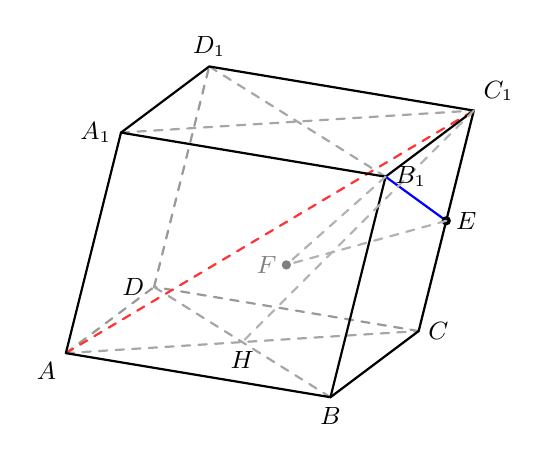
\begin{tikzpicture}[scale=1.4, >=stealth, line join=round, line cap=round]
    % 顶点坐标
    \coordinate (A) at (0,0);
    \coordinate (B) at (2.4,-0.4);
    \coordinate (D) at (0.8,0.6);
    \coordinate (C) at (3.2,0.2);
    
    \coordinate (A1) at (0.5,2.0);
    \coordinate (B1) at (2.9,1.6);
    \coordinate (D1) at (1.3,2.6);
    \coordinate (C1) at (3.7,2.2);
    
    \coordinate (E) at ($(C1)!0.5!(C)$); % 侧棱 CC1 上的点 E
    
    % 隐藏线（背面）
    \draw[dashed, thick, gray!80] (A) -- (D);
    \draw[dashed, thick, gray!80] (C) -- (D);
    \draw[dashed, thick, gray!80] (D) -- (D1);
    \draw[dashed, thick, gray!70] (A) -- (C);
    \draw[dashed, thick, gray!70] (B) -- (D);
    \draw[dashed, thick, gray!70] (A1) -- (C1);
    \draw[dashed, thick, gray!70] (B1) -- (D1);
    \draw[dashed, thick, red!80] (A) -- (C1);
    
    % 可见实线
    \draw[thick] (A) -- (B) -- (C) -- (C1) -- (D1) -- (A1) -- cycle;
    \draw[thick] (B) -- (B1) -- (C1);
    \draw[thick] (A1) -- (B1);
    \draw[thick, blue] (B1) -- (E);
    
    \fill (E) circle (1.2pt) node[right] {\small $E$};
    
    % 辅助讲解线：垂线
    \coordinate (H) at (1.6,0.1); % AC 中点 H
    \draw[dashed, thick, gray!60] (C1) -- (H);
    \node[below] at (H) {\small $H$};
    
    \coordinate (E0) at (2.0,0.8);
    \fill[gray] (E0) circle (1.2pt) node[left] {\small $F$};
    \draw[dashed, thick, gray!60] (E) -- (E0);
    \draw[dashed, thick, gray!60] (B1) -- (E0);
    
    \node[below left] at (A) {\small $A$};
    \node[below] at (B) {\small $B$};
    \node[right] at (C) {\small $C$};
    \node[left] at (D) {\small $D$};
    \node[left] at (A1) {\small $A_1$};
    \node[right] at (B1) {\small $B_1$};
    \node[above right] at (C1) {\small $C_1$};
    \node[above] at (D1) {\small $D_1$};
\end{tikzpicture}
\end{center}

\subsection{几何证明与解析}

\begin{proof*}[第（1）问：证明 $AA_1 \perp B_1D_1$]
在顶面菱形 $A_1B_1C_1D_1$ 中，有 $A_1B_1 = A_1D_1 = 2$。\par
在 $\triangle AA_1B_1$ 与 $\triangle AA_1D_1$ 中：
\[
\begin{cases}
    AA_1 = AA_1 & (\text{公共边}) \\
    A_1B_1 = A_1D_1 = 2 & (\text{菱形邻边相等}) \\
    \angle AA_1B_1 = \angle AA_1D_1 & (\text{已知角相等})
\end{cases}
\]
根据全等三角形判定定理（SAS），可知 $\triangle AA_1B_1 \cong \triangle AA_1D_1$。\par
因此有对应边相等，即 $AB_1 = AD_1$。这说明点 $A$ 到线段 $B_1D_1$ 两个端点的距离相等，所以点 $A$ 在线段 $B_1D_1$ 的垂直平分面内。\par
同时，在菱形 $A_1B_1C_1D_1$ 中，有 $A_1B_1 = A_1D_1$，即点 $A_1$ 也在线段 $B_1D_1$ 的垂直平分面内。\par
因此，直线 $AA_1$ 就在线段 $B_1D_1$ 的垂直平分面内。因为线段 $B_1D_1$ 垂直于它的垂直平分面，所以它垂直于该平面内的一切直线，故有：
\[ \boxed{AA_1 \perp B_1D_1} \]
\end{proof*}

\begin{proof*}[第（2）问：求点 $E$ 到平面 $AA_1B_1B$ 的距离]
因为侧棱 $CC_1 \parallel AA_1$，且 $AA_1$ 包含于平面 $AA_1B_1B$，所以侧棱 $CC_1$ 平行于平面 $AA_1B_1B$。\par
由于动点 $E$ 在侧棱 $CC_1$ 上，所以无论 $E$ 点如何移动，它到平面 $AA_1B_1B$ 的距离都保持不变，即等于这两个平行侧面之间的距离 $d$。下面利用等体积法进行求解。\par

首先，求解四棱柱的体积 $V$：\par
底面菱形 $ABCD$ 的面积为：
\[ S_{ABCD} = AB \cdot AD \cdot \sin 60^\circ = 2 \cdot 2 \cdot \frac{\sqrt{3}}{2} = 2\sqrt{3} \]
底面对角线 $AC = 2\sqrt{3}$，顶面对角线 $A_1C_1 = 2\sqrt{3}$。\par
在对角截面三角形 $\triangle AA_1C_1$ 中，已知三边长为 $AA_1 = 2$，$AC_1 = 2$，$A_1C_1 = 2\sqrt{3}$。由余弦定理有：
\[ \cos\angle AA_1C_1 = \frac{AA_1^2 + A_1C_1^2 - AC_1^2}{2 \cdot AA_1 \cdot A_1C_1} = \frac{4 + 12 - 4}{8\sqrt{3}} = \frac{\sqrt{3}}{2} \]
由此可得：
\[ \angle AA_1C_1 = 30^\circ \]
因为 $B_1D_1 \perp A_1C_1$ 且 $B_1D_1 \perp AA_1$（已证），所以对角线 $B_1D_1$ 垂直于对角截面 $AA_1C_1C$。\par
又因为 $B_1D_1$ 平行于底面，所以对角截面 $AA_1C_1C$ 垂直于底面，由此可知 $A_1C_1$ 即为侧棱 $AA_1$ 在顶面上的射影，则侧棱与底面所成的角为 $\angle AA_1C_1 = 30^\circ$。\par
四棱柱的高为：
\[ h = AA_1 \cdot \sin 30^\circ = 2 \cdot \frac{1}{2} = 1 \]
由此求得四棱柱的体积为：
\[ V = S_{ABCD} \cdot h = 2\sqrt{3} \cdot 1 = 2\sqrt{3} \]

其次，求解侧面 $AA_1B_1B$ 的面积：\par
侧面为平行四边形，两邻边长为 $AB = 2, AA_1 = 2$。\par
根据斜影投影关系，侧棱与底边的夹角 $\angle AA_1B_1$ 满足：
\[ \cos\angle AA_1B_1 = \cos\angle(AA_1, A_1C_1) \cdot \cos\angle(A_1C_1, A_1B_1) \]
在顶面菱形中，$A_1C_1$ 平分 $\angle D_1A_1B_1 = 60^\circ$，所以 $\angle C_1A_1B_1 = 30^\circ$。代入数据得：
\[ \cos\angle AA_1B_1 = \cos 30^\circ \cdot \cos 30^\circ = \frac{3}{4} \]

\vspace{0.2cm}
\noindent\textbf{【核心工具解析：三余弦定理（斜影投影关系）】}\par
“斜影投影关系”是立体几何中非常经典的\textbf{三余弦定理}。为了便于同学们课后彻底掌握这一工具，我们在此给出详细的推导与几何解释：

\begin{enumerate}
    \item \textbf{定理内容}：
    设直线 $l$ 是平面 $\alpha$ 的斜线，它与平面 $\alpha$ 所成的角为 $\theta_1$（即 $l$ 与它在平面 $\alpha$ 内的射影 $l'$ 的夹角）。若平面 $\alpha$ 内有一条直线 $m$ 过斜足，且 $m$ 与射影 $l'$ 的夹角为 $\theta_2$，则斜线 $l$ 与平面内直线 $m$ 的夹角 $\theta$ 满足：
    \[ \cos\theta = \cos\theta_1 \cdot \cos\theta_2 \]
    在本题中，斜线为侧棱 $AA_1$，平面为顶面 $A_1B_1C_1D_1$。由于对角截面 $AA_1C_1C \perp$ 顶面 $A_1B_1C_1D_1$，所以侧棱 $AA_1$ 在顶面上的正投影就是对角线 $A_1C_1$。顶面上的直线为 $A_1B_1$。
    因此有：$\theta = \angle AA_1B_1$，$\theta_1 = \angle AA_1C_1 = 30^\circ$，$\theta_2 = \angle C_1A_1B_1 = 30^\circ$。
    
    \item \textbf{几何证明（三垂线定理法）}：
    
    如下图所示，设斜线 $l$ 上一点为 $P$，其在平面 $\alpha$ 上的正射影为 $Q$，直线 $m$ 为平面内过斜足 $A_1$ 的直线，作 $QR \perp m$ 于 $R$，连接 $PR$。
    
    \begin{center}
    \begin{tikzpicture}[scale=1.8, >=stealth, line join=round, line cap=round]
        % 定义平面 alpha (平行四边形)
        \coordinate (P1) at (-0.5,-0.6);
        \coordinate (P2) at (4.0,-0.6);
        \coordinate (P3) at (5.0,1.3);
        \coordinate (P4) at (0.5,1.3);
        \draw[thick, fill=gray!5] (P1) -- (P2) -- (P3) -- (P4) -- cycle;
        \node[right] at (P3) {平面 $\alpha$};
        
        % 定义斜足 A1 (作为原点)
        \coordinate (A1) at (1,0);
        \node[left] at (A1) {$A_1$};
        
        % 定义各点坐标
        \coordinate (Q) at (3.5,0.7);
        \coordinate (P) at (3.5,2.1);
        \coordinate (R) at (2.6,-0.25);
        
        % 绘制线条
        \draw[thick, dashed, gray!80] (A1) -- (Q);
        \draw[thick, ->] (A1) -- ($(A1)!1.6!(Q)$) node[above] {射影 $l'$};
        
        \draw[thick] (A1) -- (P);
        \draw[thick, ->] (A1) -- ($(A1)!1.6!(P)$) node[above right] {斜线 $l$};
        
        \draw[thick] (A1) -- (R);
        \draw[thick, ->] (A1) -- ($(A1)!1.7!(R)$) node[below right] {直线 $m$};
        
        \draw[thick, dashed, red] (P) -- (Q);
        \draw[thick, dashed, blue] (Q) -- (R);
        \draw[thick, blue] (P) -- (R);
        
        \fill (Q) circle (1.2pt) node[below right] {$Q$};
        \fill (P) circle (1.2pt) node[above] {$P$};
        \fill (R) circle (1.2pt) node[below] {$R$};
        
        % 绘制直角符号
        % 1. Q 处直角 (PQ \perp A1Q)
        \draw[red] ($(Q)!0.12!(A1)$) -- ($($(Q)!0.12!(A1)$) + (0, 0.12)$) -- ($(Q) + (0, 0.12)$);
              
        % 2. R 处平面内直角 (QR \perp A1R)
        \draw[blue] ($(R)!0.12!(A1)$) -- ($($(R)!0.12!(A1)$) + ($(R)!0.12!(Q)$) - (R)$) -- ($(R)!0.12!(Q)$);
              
        % 3. R 处空间直角 (PR \perp A1R)
        \draw[blue] ($(R)!0.12!(A1)$) -- ($($(R)!0.12!(A1)$) + ($(R)!0.12!(P)$) - (R)$) -- ($(R)!0.12!(P)$);
    
        % 绘制角弧度
        \draw[->, red, thick] ($(A1)+(15.6:0.6)$) arc (15.6:40:0.6);
        \node[red, right] at ($(A1)+(27.8:0.65)$) {$\theta_1$};
        
        \draw[->, blue, thick] ($(A1)+(-8.9:0.8)$) arc (-8.9:15.6:0.8);
        \node[blue, right] at ($(A1)+(3.3:0.85)$) {$\theta_2$};
        
        \draw[->, black, thick] ($(A1)+(-8.9:0.4)$) arc (-8.9:40:0.4);
        \node[black, left, shift={(-0.05, 0.1)}] at ($(A1)+(15.6:0.35)$) {$\theta$};
    \end{tikzpicture}
    \end{center}
    
    在斜线 $l$ 上取一点 $P$，作 $PQ \perp \text{平面 } \alpha$ 于点 $Q$，则点 $Q$ 落在射影 $l'$ 上，且 $\triangle PQA_1$ 为直角三角形（$\angle PQA_1 = 90^\circ$），有：
    \[ A_1Q = A_1P \cdot \cos\theta_1 \]
    在平面 $\alpha$ 内，作 $QR \perp m$ 于点 $R$，连接 $PR$。
    因为 $PQ \perp \text{平面 } \alpha$，且 $QR \perp m$，根据三垂线定理，斜线 $PR \perp m$。
    因此，$\triangle PRA_1$ 和 $\triangle QRA_1$ 均为直角三角形（$\angle PRA_1 = 90^\circ, \angle QRA_1 = 90^\circ$）。
    在直角三角形 $\triangle QRA_1$ 中，有：
    \[ A_1R = A_1Q \cdot \cos\theta_2 \]
    在直角三角形 $\triangle PRA_1$ 中，有：
    \[ A_1R = A_1P \cdot \cos\theta \]
    将第一步的 $A_1Q$ 代入，得：
    \[ A_1R = (A_1P \cdot \cos\theta_1) \cdot \cos\theta_2 \]
    结合 $A_1R = A_1P \cdot \cos\theta$，消去 $A_1P$ 即可得到：
    \[ \cos\theta = \cos\theta_1 \cdot \cos\theta_2 \]
    
    \item \textbf{向量证明（正交分解）}：
    设斜线 $l$、射影 $l'$、平面直线 $m$ 的单位方向向量分别为 $\vec{u}, \vec{v}, \vec{w}$。
    由于 $\vec{v}$ 是 $\vec{u}$ 在平面上的投影方向，我们可以将斜线向量 $\vec{u}$ 正交分解为平行于平面的分量与垂直于平面的分量：
    \[ \vec{u} = \cos\theta_1 \vec{v} + \vec{n} \]
    其中 $\vec{n}$ 为平面 $\alpha$ 的法向量，满足 $\vec{n} \cdot \vec{v} = 0$，且 $\vec{n} \cdot \vec{w} = 0$。
    求向量 $\vec{u}$ 与 $\vec{w}$ 的数量积：
    \[ \cos\theta = \vec{u} \cdot \vec{w} = (\cos\theta_1 \vec{v} + \vec{n}) \cdot \vec{w} = \cos\theta_1 (\vec{v} \cdot \vec{w}) + \vec{n} \cdot \vec{w} \]
    由于 $\vec{v} \cdot \vec{w} = \cos\theta_2$，且 $\vec{n} \cdot \vec{w} = 0$，代入立即得到：
    \[ \cos\theta = \cos\theta_1 \cdot \cos\theta_2 \]
\end{enumerate}
掌握三余弦定理，能够帮助我们在斜棱柱或斜面中快速转换“空间斜线”、“平面内直线”和“投影线”之间的夹角，极大简化了寻找和构建直角三角形的步骤。
\vspace{0.2cm}

从而有：
\[ \sin\angle AA_1B_1 = \sqrt{1 - \left(\frac{3}{4}\right)^2} = \frac{\sqrt{7}}{4} \]
侧面 $AA_1B_1B$ 的面积为：
\[ S_{AA_1B_1B} = AB \cdot AA_1 \cdot \sin\angle AA_1B_1 = 2 \cdot 2 \cdot \frac{\sqrt{7}}{4} = \sqrt{7} \]

最后，根据体积与底面积的关系：
\[ V = S_{AA_1B_1B} \cdot d \implies 2\sqrt{3} = \sqrt{7} \cdot d \implies d = \frac{2\sqrt{21}}{7} \]
故点 $E$ 到平面 $AA_1B_1B$ 的距离为：
\[ \boxed{d(E, \text{平面 } AA_1B_1B) = \frac{2\sqrt{21}}{7}} \]
\end{proof*}

\begin{proof*}[第（3）问：求 $C_1E$ 的长度]
在第（3）问中，已知条件为线面角的正弦值，但目标量 $C_1E$ 并不在此角度所在的直角三角形中。我们需要通过直角三角形先求出中间量（斜边） $B_1E$，再平移到侧面三角形中进行消元求解。

\textbf{1. 在投影直角三角形 $\triangle B_1EF$ 中求解中间量 $B_1E$}\par
设点 $E$ 到平面 $AA_1B_1B$ 的垂足为 $F$，连接 $B_1F$。
则 $\triangle B_1EF$ 是以 $F$ 为直角顶点的直角三角形，$\angle EB_1F$ 即为斜线 $B_1E$ 与平面 $AA_1B_1B$ 所成的线面角。
如下图所示，我们将这个空间投影三角形用红色阴影标出。

\begin{center}
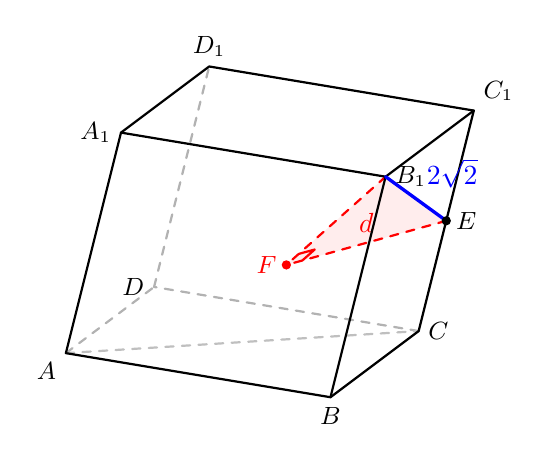
\begin{tikzpicture}[scale=1.4, >=stealth, line join=round, line cap=round]
    % 顶点坐标
    \coordinate (A) at (0,0);
    \coordinate (B) at (2.4,-0.4);
    \coordinate (D) at (0.8,0.6);
    \coordinate (C) at (3.2,0.2);
    
    \coordinate (A1) at (0.5,2.0);
    \coordinate (B1) at (2.9,1.6);
    \coordinate (D1) at (1.3,2.6);
    \coordinate (C1) at (3.7,2.2);
    
    \coordinate (E) at ($(C1)!0.5!(C)$); % 侧棱 CC1 上的点 E
    
    % F 是 E 在面 AA1B1B 上的投影
    \coordinate (F) at (2.0,0.8);
    
    % 阴影着色
    \fill[red!10, opacity=0.7] (B1) -- (E) -- (F) -- cycle;
    
    % 隐藏线
    \draw[dashed, thick, gray!60] (A) -- (D);
    \draw[dashed, thick, gray!60] (C) -- (D);
    \draw[dashed, thick, gray!60] (D) -- (D1);
    \draw[dashed, thick, gray!50] (A) -- (C);
    
    % 投影三角形内部线条
    \draw[dashed, red, thick] (E) -- (F) node[midway, above] {$d$};
    \draw[dashed, red, thick] (B1) -- (F);
    
    % 可见实线
    \draw[thick] (A) -- (B) -- (C) -- (C1) -- (D1) -- (A1) -- cycle;
    \draw[thick] (B) -- (B1) -- (C1);
    \draw[thick] (A1) -- (B1);
    \draw[thick, blue, very thick] (B1) -- (E) node[midway, above right] {$2\sqrt{2}$};
    
    % 直角标记
    \coordinate (F1) at ($(F)!0.15cm!(E)$);
    \coordinate (F2) at ($(F)!0.15cm!(B1)$);
    \coordinate (F3) at ($(F1)+(F2)-(F)$);
    \draw[red, thick] (F1) -- (F3) -- (F2);
    
    \fill (E) circle (1.2pt) node[right] {\small $E$};
    \fill[red] (F) circle (1.2pt) node[left] {\small $F$};
    
    \node[below left] at (A) {\small $A$};
    \node[below] at (B) {\small $B$};
    \node[right] at (C) {\small $C$};
    \node[left] at (D) {\small $D$};
    \node[left] at (A1) {\small $A_1$};
    \node[right] at (B1) {\small $B_1$};
    \node[above right] at (C1) {\small $C_1$};
    \node[above] at (D1) {\small $D_1$};
\end{tikzpicture}
\end{center}

已知 $\sin\angle EB_1F = \dfrac{\sqrt{42}}{14}$，且垂线段 $EF = d = \dfrac{2\sqrt{21}}{7}$。\par
在 Rt$\triangle B_1EF$ 中，根据正弦定义：
\[ \sin\angle EB_1F = \frac{EF}{B_1E} \implies \frac{\sqrt{42}}{14} = \frac{\frac{2\sqrt{21}}{7}}{B_1E} \]
解得：
\[ \boxed{B_1E = 2\sqrt{2}} \]

\textbf{2. 在侧面平面三角形 $\triangle B_1C_1E$ 中求解目标量 $C_1E$}\par
求得 $B_1E$ 之后，我们需要将计算转化至侧面平行四边形 $BCC_1B_1$ 内的三角形 $\triangle B_1C_1E$ 中。
为了便于分析，我们将侧面 $BCC_1B_1$ 作为一个平面图形单独画出，如下图所示。

\begin{center}
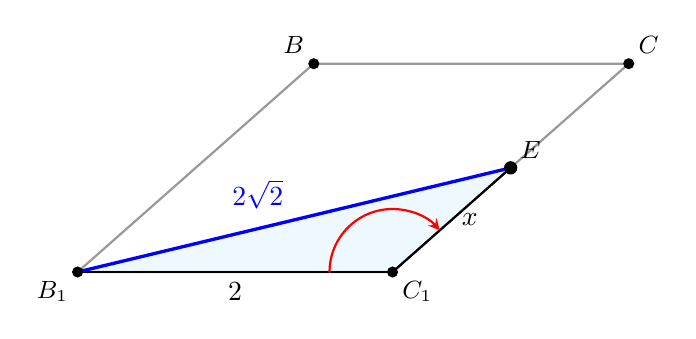
\begin{tikzpicture}[scale=2.0, >=stealth, line join=round, line cap=round]
    \coordinate (C1) at (0,0);
    \coordinate (B1) at (-2,0);
    \coordinate (C) at ({2*cos(41.41)}, {2*sin(41.41)});
    \coordinate (B) at ($(-2,0) + ({2*cos(41.41)}, {2*sin(41.41)})$);
    \coordinate (E) at ({1*cos(41.41)}, {1*sin(41.41)});
    
    % 阴影着色
    \fill[cyan!10, opacity=0.7] (B1) -- (C1) -- (E) -- cycle;
    
    \draw[thick, gray!80] (B) -- (C) -- (C1) -- (B1) -- cycle;
    
    \draw[thick, black] (B1) -- (C1) node[midway, below] {$2$};
    \draw[thick, black] (C1) -- (E) node[midway, right] {$x$};
    \draw[thick, blue, very thick] (B1) -- (E) node[midway, above left] {$2\sqrt{2}$};
    
    \draw[->, thick, red] (-0.4, 0) arc (180:41.41:0.4);
    
    \fill (C1) circle (1pt) node[below right] {\small $C_1$};
    \fill (B1) circle (1pt) node[below left] {\small $B_1$};
    \fill (C) circle (1pt) node[above right] {\small $C$};
    \fill (B) circle (1pt) node[above left] {\small $B$};
    \fill (E) circle (1.2pt) node[above right] {\small $E$};
\end{tikzpicture}
\end{center}

在平面三角形 $\triangle B_1C_1E$ 中，已知两边 $B_1C_1 = 2$ 和 $B_1E = 2\sqrt{2}$，设 $C_1E = x$。\par
因为 $C_1E \parallel AA_1$ 且 $C_1B_1 \parallel A_1D_1$，所以角 $\angle B_1C_1E$ 与角 $\angle AA_1D_1$ 互补。\par
由于 $\cos\angle AA_1D_1 = \cos\angle AA_1B_1 = \dfrac{3}{4}$。
因此：
\[ \cos\angle B_1C_1E = -\cos\angle AA_1D_1 = -\frac{3}{4} \]
在平面 $\triangle B_1C_1E$ 中，由余弦定理：
\[ B_1E^2 = B_1C_1^2 + C_1E^2 - 2 \cdot B_1C_1 \cdot C_1E \cdot \cos\angle B_1C_1E \]
代入已知数据：
\[ (2\sqrt{2})^2 = 2^2 + x^2 - 2 \cdot 2 \cdot x \cdot \left(-\frac{3}{4}\right) \]
\[ \implies 8 = 4 + x^2 + 3x \implies x^2 + 3x - 4 = 0 \]
解方程得 $(x-1)(x+4) = 0$。因为线段长度恒为正值，舍去 $x = -4$，得：
\[ \boxed{C_1E = 1} \]
\end{proof*}

\subsection{解题方法与技巧小结}
在解答此类立体几何题目时，可以总结以下方法：
\begin{enumerate}
    \item \textbf{利用全等三角形对称性简化证明} \\
    当题目中给出类似 $\angle AA_1B_1 = \angle AA_1D_1$ 的角相等条件时，可先观察侧面三角形是否全等。通过 $\triangle AA_1B_1 \cong \triangle AA_1D_1$ 得到 $AB_1 = AD_1$，进而利用垂直平分面的性质直接证明垂直关系，省去作辅助线的繁琐步骤。
    \item \textbf{动点在平行平面上滑动时距离恒定} \\
    当动点 $E$ 在与目标平面平行的直线或平面上滑动时，它到目标平面的距离为常数。这意味着可以将动点距离转化为两个平行平面之间的距离，从而把“动点”转化为“定点”处理。
    \item \textbf{利用等体积法避免直接作高} \\
    在斜棱柱等较倾斜的几何体中，点到平面的垂线段在空间中很难画出位置并加以证明。利用体积公式的“底面变换”（如 $V = S_{\text{底}} \cdot h = S_{\text{侧}} \cdot d$）可以将求高问题直接转化为体积与面积的除法运算，避开寻找垂足的环节。
    \item \textbf{线面角正弦值的直接应用} \\
    直线与平面所成的角本质上落在由斜线、投影线和垂线段组成的直角三角形中。线面角的正弦值就是点到平面的距离与斜线段长度之比，即 $\sin\theta = \frac{d}{l}$。
    \item \textbf{通过中间量进行三角形平移} \\
    在平面三角形 $\triangle B_1C_1E$ 中，已知两边，若能找到某个角，就可以用余弦定理建立方程；若找到的是两已知边的夹角，则可直接确定第三边。通过公共斜线长 $B_1E$ 作为“桥梁”，将计算平移到目标三角形中。
\end{enumerate}

\newpage
% ==================== 第二部分 ====================
\section{空间角的核心定理及其应用拓展}

在解决立体几何问题时，尤其是面对线面角、二面角和线线角相互交织的复杂空间图形时，直接利用空间辅助线作高、投影往往对空间想象力要求极高。为此，立体几何中整理出了处理空间角的一组核心定理：\textbf{三余弦定理}、\textbf{三正弦定理}、\textbf{三夹角定理}、\textbf{三射线定理} 和 \textbf{二面角三余弦定理}。它们是解决空间角计算问题的强力工具，能够帮助我们快速完成“降维”和“跨角计算”。

\noindent\textbf{【核心教学思想：空间投影与面面关系】}\par
这五个定理的本质，其实不是“五个孤立的公式”，而是两个核心思想的体现：\textbf{空间线与平面的投影转换} 以及 \textbf{面与面之间的夹角控制}。

根据研究对象，我们可以将这五个定理分为两类：
\begin{enumerate}
    \item \textbf{第一类：一条线和一个平面的关系（空间线 $\longrightarrow$ 投影到平面）}
    \begin{itemize}
        \item \textbf{三余弦定理}：已知线面角和影子方向，求斜线与底面某直线的夹角。看的是“斜线和影子”。
        \item \textbf{三夹角定理}：已知空间线与底面内两条基准直线的夹角，反求线面角。用的是“三条棱求线面角”。
    \end{itemize}
    \item \textbf{第二类：两个平面的关系（两个面 $\longrightarrow$ 各自内部直线的夹角与面面角的关系）}
    \begin{itemize}
        \item \textbf{三正弦定理}：已知二面角和斜面内斜线方向，求该斜线与底面的线面角。看的是“斜坡和走向”。
        \item \textbf{二面角三余弦定理}：已知二面角及两个平面内直线与交线的夹角，求两直线的夹角。看的是“面内直线与交线”。
        \item \textbf{三射线定理}：已知从同一点出发的三条射线两两夹角，求两个面的二面角。用的是“三条棱求二面角”（本质上是二面角三余弦定理的直接变形）。
    \end{itemize}
\end{enumerate}

最适合学生记忆的口诀是：
\begin{center}
\textbf{三余弦看“斜线和影子”；三正弦看“斜坡和走向”；\\
三夹角用“三条棱求线面角”；三射线与二面角三余弦看“两个面内线的张角”。}
\end{center}
这比直接背公式更加稳定。公式只是最后的计算工具，而几何模型才是学生在考场上能够灵活迁移的本质。


\subsection{三余弦定理（最小角定理）}

\begin{theorembox}{三余弦定理（最小角定理）}
设直线 $OP$ 是平面 $\alpha$ 的斜线，斜足为 $O$，点 $P$ 在平面 $\alpha$ 上的正投影为 $H$（即 $PH \perp \text{平面 } \alpha$）。在平面 $\alpha$ 内任取一条过斜足 $O$ 的直线 $OQ$。\\
记：
\begin{itemize}
    \item $\theta = \angle POH$ 为斜线 $OP$ 与平面 $\alpha$ 所成的线面角（即“竖直角”）；
    \item $\beta = \angle HOK$ 为投影线 $OH$ 与底面内直线 $OQ$ 的夹角（即“水平角”）；
    \item $\gamma = \angle POK$ 为斜线 $OP$ 与底面内直线 $OQ$ 的夹角（即“斜角”）。
\end{itemize}
则这三个角满足如下余弦关系式：
\[ \cos\gamma = \cos\theta \cos\beta \]
即：
\[ \cos(\text{斜角}) = \cos(\text{线面角}) \cos(\text{水平角}) \]
因为在区间 $\left[0, \frac{\pi}{2}\right]$ 内，$\cos\beta \le 1 \implies \cos\gamma \le \cos\theta \implies \gamma \ge \theta$。这说明线面角是斜线与平面内所有直线所成角中的最小角，因此也称为\textbf{最小角定理}。
\end{theorembox}

\noindent\textbf{【模型剖析与学生应用】}
\begin{itemize}
    \item \textbf{模型本质：斜线看地面方向} \\
    斜线和地面上一条线的夹角，由两部分共同决定：\textbf{斜线离开地面的角度（线面角）} $+$ \textbf{影子在地面里偏开的角度（平面内投影角）}。
    \item \textbf{给学生的说法} \\
    “你看一根斜着插在地上的杆子。它和地上一条线的夹角，不只看杆子有多陡，还要看杆子的影子和这条地面线偏了多少。”
    \item \textbf{统一模型} \\
    \[ \text{空间斜角} \Rightarrow \text{线面角} + \text{平面内投影角} \quad (\text{余弦值相乘}) \]
    它也解释了为什么\textbf{线面角最小}：当地面线 $OQ$ 与投影线 $OH$ 完全重合时，$\beta = 0^\circ$，此时 $\cos\beta = 1$，$\gamma = \theta$ 达到最小。偏离投影线越远，$\beta$ 越大，$\cos\beta$ 越小，从而 $\cos\gamma$ 越小，空间斜角 $\gamma$ 越大。
\end{itemize}


\begin{center}
\begin{tikzpicture}[scale=2.0, >=stealth, line join=round, line cap=round]
    % 定义交点 O
    \coordinate (O) at (0,0);
    \node[below left] at (O) {$O$};
    
    % 平面 \alpha (斜投影平行四边形)
    \coordinate (A1) at (-1.8,-0.8);
    \coordinate (A2) at (2.8,-0.8);
    \coordinate (A3) at (4.0,1.2);
    \coordinate (A4) at (-0.6,1.2);
    \draw[thick, gray!50] (A1) -- (A2) -- (A3) -- (A4) -- cycle;
    \node[right] at (A3) {平面 $\alpha$ (地面)};
    
    % 点 P (在平面上方)
    \coordinate (P) at (1.8, 2.2);
    \fill (P) circle (1.2pt) node[above] {$P$};
    
    % 点 H (P 在平面上的正投影)
    \coordinate (H) at (1.8, 0.6);
    \fill (H) circle (1.2pt) node[below right] {$H$};
    
    % 连线 OP, OH, PH
    \draw[thick, black] (O) -- (P) node[midway, above left, scale=0.8] {斜线};
    \draw[thick, dashed, red] (P) -- (H);
    \draw[thick, dashed, red] (O) -- (H) node[midway, below, scale=0.8, shift={(0.1,-0.05)}] {影子};
    
    % 直线 OQ (在平面内)
    \coordinate (Q) at (2.5, -0.5);
    \draw[thick, blue] (O) -- ($(O)!1.2!(Q)$) node[midway, below, scale=0.8, sloped] {地面方向} node[right] {$Q$};
    
    % 从 H 向 OQ 作垂线，垂足为 K
    % K 的坐标经过精确投影计算：t = 4.2/6.5 = 0.646 -> K = (1.615, -0.323)
    \coordinate (K) at (1.615, -0.323);
    \fill (K) circle (1.2pt) node[below left] {$K$};
    \draw[thick, dashed, blue] (H) -- (K);
    
    % 连接 PK
    \draw[thick, blue] (P) -- (K);
    
    % 绘制直角标记
    % PH \perp OH
    \draw[red] ($(H)!0.1!(P)$) -- ($($(H)!0.1!(P)$) + ($(H)!0.1!(O)$) - (H)$) -- ($(H)!0.1!(O)$);
    % HK \perp OK
    \draw[blue] ($(K)!0.1!(H)$) -- ($($(K)!0.1!(H)$) + ($(K)!0.1!(O)$) - (K)$) -- ($(K)!0.1!(O)$);
    % PK \perp OK (由三垂线定理)
    \draw[blue] ($(K)!0.1!(P)$) -- ($($(K)!0.1!(P)$) + ($(K)!0.1!(O)$) - (K)$) -- ($(K)!0.1!(O)$);
    
    % 标记角
    % \theta = \angle POH (线面角)
    \draw[->, red, thick] ($(O)+(18.43:0.5)$) arc (18.43:50.71:0.5);
    \node[red, right] at ($(O)+(34.57:0.55)$) {$\theta$};
    
    % \beta = \angle HOK (投影夹角)
    \draw[->, blue, thick] ($(O)+(-11.31:0.4)$) arc (-11.31:18.43:0.4);
    \node[blue, right] at ($(O)+(3.56:0.45)$) {$\beta$};
    
    % \gamma = \angle POK (斜线与 OQ 夹角)
    \draw[->, purple, thick] ($(O)+(-11.31:0.8)$) arc (-11.31:50.71:0.8);
    \node[purple, above right] at ($(O)+(25:0.85)$) {$\gamma$};
\end{tikzpicture}
\end{center}

\noindent\textbf{2. 定理证明}\par
在平面 $\alpha$ 内，过点 $H$ 作 $HK \perp OQ$ 于点 $K$，连接 $PK$。\\
因为 $PH \perp \text{平面 } \alpha$，且 $OQ \subset \text{平面 } \alpha$，所以 $PH \perp OQ$。\\
又 $HK \perp OQ$，且 $PH \cap HK = H$，所以 $OQ \perp \text{平面 } PHK$。\\
因为 $PK \subset \text{平面 } PHK$，所以 $OQ \perp PK$，即 $PK \perp OQ$。\\
在直角三角形 $\triangle POK$ 中（$\angle PKO = 90^\circ$），有：
\[ \cos\gamma = \cos\angle POK = \frac{OK}{OP} \]
在直角三角形 $\triangle HOK$ 中（$\angle HKO = 90^\circ$），有：
\[ OK = OH \cos\beta \]
在直角三角形 $\triangle POH$ 中（$\angle PHO = 90^\circ$），有：
\[ OH = OP \cos\theta \]
将上述关系代入，得：
\[ OK = OP \cos\theta \cos\beta \implies \frac{OK}{OP} = \cos\theta \cos\beta \]
从而证得最小角定理的代数关系式：
\[ \cos\gamma = \cos\theta \cos\beta \]

\subsection{三正弦定理（最大角定理）}

\begin{theorembox}{三正弦定理（最大角定理）}
设两个平面 $\alpha, \beta$ 交于直线 $l$。在平面 $\alpha$ 内取一条斜线 $m$。\\
记：
\begin{itemize}
    \item $\varphi = \angle(\alpha, \beta)$ 为平面 $\alpha$ 与 $\beta$ 所成的二面角（即“面面角”）；
    \item $\lambda = \angle(m, l)$ 为平面 $\alpha$ 内的斜线 $m$ 与交线 $l$ 的夹角（即“线线角”）；
    \item $\omega = \angle(m, \beta)$ 为斜线 $m$ 与平面 $\beta$ 所成的线面角。
\end{itemize}
则这三个角满足如下正弦关系式：
\[ \sin\omega = \sin\varphi \sin\lambda \]
即：
\[ \sin(\text{线面角}) = \sin(\text{面面角}) \sin(\text{线线角}) \]
由于 $0 \le \sin\lambda \le 1$，所以 $\sin\omega \le \sin\varphi$。在锐角范围内有 $\omega \le \varphi$，即平面内任意一条斜线与另一个平面所成的线面角，不超过这两个平面的二面角。二面角是此类线面角中的最大角，因此也称为\textbf{最大角定理}。
\end{theorembox}

\noindent\textbf{【模型剖析与学生应用】}
\begin{itemize}
    \item \textbf{模型本质：面面角控制线面角} \\
    一条线如果躺在斜面上，它离开底面的程度（线面角），取决于两个因素：\textbf{这个斜面本身有多陡（二面角）} $+$ \textbf{这条线在斜面里是否朝着“最陡方向”走（线线角）}。
    \item \textbf{给学生的说法} \\
    “斜坡有一个最大坡度。你如果沿着最陡方向往上走，坡度最大；如果斜着走，实际爬升角就变小；如果沿着等高线走，角度就是 0。”
    \item \textbf{统一模型} \\
    \[ \text{线面角} \Rightarrow \text{二面角} \times \text{这条线偏离交线的程度} \quad (\text{正弦值相乘}) \]
    它也解释了为什么\textbf{二面角最大}：当斜线 $m$ 垂直于交线 $l$ 时，$\lambda = 90^\circ$，$\sin\lambda = 1$，此时线面角 $\omega$ 达到最大，等于二面角 $\varphi$。
\end{itemize}


\begin{center}
\begin{tikzpicture}[scale=2.2, >=stealth, line join=round, line cap=round]
    % 定义交线上的点 O 作为垂心位置的投影点
    \coordinate (O) at (0.6,0);
    \node[below] at (O) {$O$};
    
    % 定义交线 l (沿 x 轴方向)
    \draw[thick, black] (-3.0,0) -- (3.0,0) node[right] {交线 $l$};
    \coordinate (Q) at (-1.2,0);
    \fill (Q) circle (1.2pt) node[below] {$Q$};
    
    % 平面 beta (底面, 用平行四边形表示，体现同向向后延伸的透视效果)
    \coordinate (B1) at (-2.0,0);
    \coordinate (B2) at (-1.2,0.8);
    \coordinate (B3) at (2.8,0.8);
    \coordinate (B4) at (2.0,0);
    \draw[thick, gray!50] (B1) -- (B2);
    \draw[thick, gray!50, dashed] (B2) -- (B3);
    \draw[thick, gray!50] (B3) -- (B4);
    \node[below right] at (B3) {底面 $\beta$ (地面)};
    
    % 平面 alpha (斜面, 同向向后上方斜立延伸，与底面形成清晰的“夹角”空间)
    \coordinate (A1) at (-2.0,0);
    \coordinate (A2) at (-1.2,1.6);
    \coordinate (A3) at (2.8,1.6);
    \coordinate (A4) at (2.0,0);
    \draw[thick, gray!70] (A1) -- (A2) -- (A3) -- (A4);
    \node[above left] at (A2) {斜面 $\alpha$ (斜坡)};
    
    % 在面 alpha 内定义点 P (x=1.2, y=1.4)
    \coordinate (P) at (1.2,1.4);
    \fill (P) circle (1.2pt) node[above] {$P$};
    
    % PO (平面内垂直于交线的线段)
    \draw[thick, blue] (P) -- (O);
    
    % 从 P 向面 beta 作垂线，垂足为 H (x=1.2, y=0.6)
    \coordinate (H) at (1.2,0.6);
    \fill (H) circle (1.2pt) node[right] {$H$};
    \draw[thick, dashed, red] (P) -- (H);
    
    % 连接 OH (投影线, 保持虚线表示其在平面内部的投影性质)
    \draw[thick, dashed, red] (O) -- (H);
    
    % 斜线 m (在面 alpha 内从 Q 出发经过 P)
    \draw[thick, blue] (Q) -- (P);
    \draw[thick, ->, blue] (P) -- ($(Q)!1.4!(P)$) node[above right] {斜线 $m$ (走向)};
    
    % 连接 QH (m 在平面 beta 内的投影，虚线)
    \draw[thick, dashed, purple] (Q) -- (H);
    
    % 绘制直角符号
    % 1. PO \perp l 于 O
    \draw[blue] ($(O)!0.12!(P)$) -- ($($(O)!0.12!(P)$) + ($(O)!0.12!(Q)$) - (O)$) -- ($(O)!0.12!(Q)$);
    % 2. OH \perp l 于 O
    \draw[red] ($(O)!0.12!(H)$) -- ($($(O)!0.12!(H)$) + ($(O)!0.12!(Q)$) - (O)$) -- ($(O)!0.12!(Q)$);
    % 3. PH \perp beta 于 H, 故 PH \perp OH
    \draw[red] ($(H)!0.1!(P)$) -- ($($(H)!0.1!(P)$) + ($(H)!0.1!(O)$) - (H)$) -- ($(H)!0.1!(O)$);
    
    % 标记角度
    % 面面角 \varphi = \angle POH (二面角)
    \draw[->, red, thick] ($(O)+(45:0.3)$) arc (45:66.8:0.3);
    \node[red, above right, shift={(-0.02,-0.02)}] at ($(O)+(55:0.35)$) {$\varphi$};
    
    % 线线角 \lambda = \angle PQO
    \draw[->, blue, thick] ($(Q)+(0:0.45)$) arc (0:30.3:0.45);
    \node[blue, above right] at ($(Q)+(15:0.52)$) {$\lambda$};
    
    % 线面角 \omega = \angle PQH
    \draw[->, purple, thick] ($(Q)+(14.0:0.65)$) arc (14.0:30.3:0.65);
    \node[purple, right] at ($(Q)+(22:0.72)$) {$\omega$};
\end{tikzpicture}
\end{center}

\noindent\textbf{2. 定理证明}\par
如上图所示，在平面 $\alpha$ 内取一点 $P$，作 $PO \perp l$ 于点 $O$。从点 $P$ 向平面 $\beta$ 作垂线 $PH \perp \beta$ 于点 $H$，连接 $OH$。\\
由三垂线定理的逆定理，可知 $OH \perp l$。因此，$\angle POH = \varphi$ 就是平面 $\alpha$ 与平面 $\beta$ 所成的二面角。\\
在平面 $\alpha$ 内另取一条直线 $m$（即射线 $PQ$），与交线 $l$ 交于点 $Q$，连接 $QH$。由于 $PH \perp \text{平面 } \beta$，可知直线 $m$ 与平面 $\beta$ 所成的线面角为 $\omega = \angle PQH$。\\
此时：
\begin{itemize}
    \item 线线角 $\lambda = \angle PQO$，在直角三角形 $\triangle POQ$ 中，有 $\sin\lambda = \dfrac{PO}{PQ}$；
    \item 二面角 $\varphi = \angle POH$，在直角三角形 $\triangle POH$ 中，有 $\sin\varphi = \dfrac{PH}{PO}$；
    \item 线面角 $\omega = \angle PQH$，在直角三角形 $\triangle PQH$ 中，有 $\sin\omega = \dfrac{PH}{PQ}$。
\end{itemize}
将两式相乘：
\[ \sin\varphi \sin\lambda = \frac{PH}{PO} \cdot \frac{PO}{PQ} = \frac{PH}{PQ} = \sin\omega \]
即证得最大角定理的代数关系式：
\[ \sin\omega = \sin\varphi \sin\lambda \]

\subsection{三夹角定理}

\begin{theorembox}{三夹角定理}
设从同一点 $A$ 引出三条射线 $AB, AC, AD$，其中 $AB, AC$ 确定平面 $ABC$，$AD$ 是空间中的另一条射线。\\
记三条射线两两夹角为：
\[ \alpha = \angle BAC, \quad \beta = \angle BAD, \quad \gamma = \angle CAD \]
设直线 $AD$ 与平面 $ABC$ 所成的线面角为 $\theta$，则有：
\[ \cos\theta = \frac{\sqrt{\cos^2\beta + \cos^2\gamma - 2\cos\alpha \cos\beta \cos\gamma}}{\sin\alpha} \]
该定理适合在已知三条射线两两夹角时，快速求出其中一条射线与另外两条射线所在平面的线面角。
\end{theorembox}

\noindent\textbf{【模型剖析与学生应用】}
\begin{itemize}
    \item \textbf{模型本质：三条棱确定一条线对底面的倾斜} \\
    已知空间射线 $AD$ 与底面内两条基准线 $AB, AC$ 的夹角，就可以确定 $AD$ 在底面上的投影长度，从而求出它离开底面的角度。其本质是\textbf{向量投影}：把 $AD$ 投影到平面 $ABC$ 上，再用 $AB, AC$ 这两个底面不平行方向（基底向量）表示该投影。
    \item \textbf{给学生的说法} \\
    “如果你知道一根空间斜线分别和地面上两条不平行方向的夹角，那么它的影子在地面上的方向和长度就被确定了。影子越长（离底面越贴近），线面角越小；影子越短，线面角越大。”
    \item \textbf{统一模型} \\
    \[ \text{两条底面方向} + \text{空间线与它们的夹角} \Rightarrow \text{空间线与底面的夹角} \]
\end{itemize}


\begin{center}
\begin{tikzpicture}[scale=2.0, >=stealth, line join=round, line cap=round]
    % 定义底面平面 ABC (用平行四边形边框表示，被遮挡的后半部分用虚线绘制)
    \coordinate (P1) at (-0.8,-0.8);
    \coordinate (P2) at (3.6,-0.8);
    \coordinate (P3) at (4.4,1.0);
    \coordinate (P4) at (0.0,1.0);
    
    % 1. 前半部分边界 (实线)
    \draw[thick, gray!50] (-0.44, 0) -- (P1) -- (P2) -- (3.96, 0);
    \node[below right] at (P3) {平面 $ABC$};
    
    % 2. 后半部分边界 (被空间射线和平面遮挡，用虚线表示)
    \draw[thick, gray!50, dashed] (3.96, 0) -- (P3) -- (P4) -- (-0.44, 0);

    % 定义顶点 A (原点)
    \coordinate (A) at (0,0);
    \node[left, shift={(-0.05,0)}] at (A) {$A$};
    
    % 定义底面内射线 AB, AC
    \coordinate (B) at (3.0,-0.6);
    \coordinate (C) at (2.4,0.8);
    \draw[thick, ->, black] (A) -- (B) node[below right] {$B$};
    \draw[thick, ->, black] (A) -- (C) node[above right] {$C$};
    
    % 定义空间射线 AD
    \coordinate (D) at (2.0,1.8);
    \fill (D) circle (1.2pt) node[above] {$D$};
    \draw[thick, ->, black] (A) -- (D);
    
    % 从 D 向底面作垂线，垂足为 H (x 轴坐标与 D 相同，实现完全铅直的 3D 高度线)
    \coordinate (H) at (2.0,0.1);
    \fill (H) circle (1.2pt) node[below right] {$H$};
    \draw[thick, dashed, red] (D) -- (H);
    
    % 连接 AH (投影线)
    \draw[thick, dashed, red] (A) -- (H);
    
    % 绘制直角标记 DH \perp AH
    \draw[red] ($(H)!0.1!(D)$) -- ($($(H)!0.1!(D)$) + ($(H)!0.1!(A)$) - (H)$) -- ($(H)!0.1!(A)$);
    
    % 标记角
    % 1. 线面角 \theta = \angle DAH
    \draw[->, red, thick] ($(A)+(2.86:0.6)$) arc (2.86:42.0:0.6);
    \node[red, right] at ($(A)+(22.4:0.65)$) {$\theta$};
    
    % 2. 面内角 \alpha = \angle BAC
    \draw[->, black, thick] ($(A)+(-11.3:0.8)$) arc (-11.3:18.43:0.8);
    \node[black, right] at ($(A)+(3.5:0.85)$) {$\alpha$};
    
    % 3. \beta = \angle BAD
    \draw[->, black, dashed] ($(A)+(-11.3:0.4)$) arc (-11.3:42.0:0.4);
    \node[black, right, shift={(-0.02, 0.08)}] at ($(A)+(15.3:0.45)$) {$\beta$};
    
    % 4. \gamma = \angle CAD
    \draw[->, black, dashed] ($(A)+(18.43:0.5)$) arc (18.43:42.0:0.5);
    \node[black, above right] at ($(A)+(30.2:0.52)$) {$\gamma$};
\end{tikzpicture}
\end{center}

\noindent\textbf{2. 定理证明}\par
设点 $D$ 为空间射线 $AD$ 上任意一点（不同于点 $A$），点 $D$ 在底面平面 $ABC$ 上的正投影为 $H$（即 $DH \perp \text{平面 } ABC$）。\\
连接 $AH$，则 $\theta = \angle DAH$ 即为射线 $AD$ 与底面平面 $ABC$ 所成的线面角。\\
在底面 $ABC$ 内，正投影线 $AH$ 将底面角 $\angle BAC = \alpha$ 分为两部分，分别记为：
\[ \alpha_1 = \angle BAH, \quad \alpha_2 = \angle CAH \]
由平面内角度的和差关系，有：
\[ \alpha_1 + \alpha_2 = \alpha \]
根据三余弦定理（最小角定理），在空间直角三角形和投影模型中，我们有：
\begin{itemize}
    \item 对于斜线 $AD$、投影线 $AH$ 以及底面方向射线 $AB$，其线面角为 $\theta$，水平面内射影夹角为 $\alpha_1$，斜线与底面线夹角为 $\beta$。因此满足：
    \[ \cos\beta = \cos\theta \cos\alpha_1 \implies \cos\alpha_1 = \frac{\cos\beta}{\cos\theta} \quad \text{—— 方程 (1)} \]
    \item 对于斜线 $AD$、投影线 $AH$ 以及底面方向射线 $AC$，其线面角为 $\theta$，水平面内射影夹角为 $\alpha_2$，斜线与底面线夹角为 $\gamma$。因此满足：
    \[ \cos\gamma = \cos\theta \cos\alpha_2 \implies \cos\alpha_2 = \frac{\cos\gamma}{\cos\theta} \quad \text{—— 方程 (2)} \]
\end{itemize}
由三角函数的和角公式：
\[ \cos\alpha = \cos(\alpha_1 + \alpha_2) = \cos\alpha_1 \cos\alpha_2 - \sin\alpha_1 \sin\alpha_2 \]
移项整理可得：
\[ \sin\alpha_1 \sin\alpha_2 = \cos\alpha_1 \cos\alpha_2 - \cos\alpha \]
对两边平方，得：
\[ \sin^2\alpha_1 \sin^2\alpha_2 = (\cos\alpha_1 \cos\alpha_2 - \cos\alpha)^2 \]
利用平方同角三角函数关系 $\sin^2 x = 1 - \cos^2 x$ 展开左边：
\[ (1 - \cos^2\alpha_1)(1 - \cos^2\alpha_2) = \cos^2\alpha_1 \cos^2\alpha_2 - 2\cos\alpha \cos\alpha_1 \cos\alpha_2 + \cos^2\alpha \]
\[ 1 - \cos^2\alpha_1 - \cos^2\alpha_2 + \cos^2\alpha_1 \cos^2\alpha_2 = \cos^2\alpha_1 \cos^2\alpha_2 - 2\cos\alpha \cos\alpha_1 \cos\alpha_2 + \cos^2\alpha \]
消去等式两边的公共项 $\cos^2\alpha_1 \cos^2\alpha_2$，移项整理得到：
\[ \cos^2\alpha_1 + \cos^2\alpha_2 - 2\cos\alpha \cos\alpha_1 \cos\alpha_2 = 1 - \cos^2\alpha = \sin^2\alpha \]
现在，将方程 (1) 和 (2) 中关于 $\cos\alpha_1$ 和 $\cos\alpha_2$ 的表达式代入上式：
\[ \frac{\cos^2\beta}{\cos^2\theta} + \frac{\cos^2\gamma}{\cos^2\theta} - 2\cos\alpha \left(\frac{\cos\beta}{\cos\theta}\right) \left(\frac{\cos\gamma}{\cos\theta}\right) = \sin^2\alpha \]
通分后，等式可化简为：
\[ \frac{1}{\cos^2\theta} \left( \cos^2\beta + \cos^2\gamma - 2\cos\alpha \cos\beta \cos\gamma \right) = \sin^2\alpha \]
由此解得：
\[ \cos^2\theta = \frac{\cos^2\beta + \cos^2\gamma - 2\cos\alpha \cos\beta \cos\gamma}{\sin^2\alpha} \]
对两边开平方根，即证得三夹角定理公式：
\[ \cos\theta = \frac{\sqrt{\cos^2\beta + \cos^2\gamma - 2\cos\alpha \cos\beta \cos\gamma}}{\sin\alpha} \]

\subsection{三射线定理}

\begin{theorembox}{三射线定理}
仍然设三条射线为 $AB, AC, AD$，两两夹角记为 $\alpha = \angle BAC, \beta = \angle BAD, \gamma = \angle CAD$。\\
设平面 $DAC$ 与平面 $BAC$ 沿公共棱 $AC$ 所成的二面角为 $\varphi$，则有：
\[ \cos\varphi = \frac{\cos\beta - \cos\alpha \cos\gamma}{\sin\alpha \sin\gamma} \]
该定理适合在已知三条射线两两夹角时，直接求出对应二面角的大小。
\end{theorembox}

\noindent\textbf{【模型剖析与学生应用】}
\begin{itemize}
    \item \textbf{模型本质：三条棱确定两个面的夹角} \\
    两个面绕着同一条公共棱 $AC$ 张开。要看它们张开多少，就分别在两个面内作垂直于公共棱 $AC$ 的方向向量，再求这两个方向向量的夹角。其本质也是\textbf{向量投影}：把 $AD$ 和 $AB$ 分别去掉沿公共棱 $AC$ 的平行分量，剩下的就是两个面内垂直于 $AC$ 的投影方向，再求这两个投影方向的夹角。
    \item \textbf{给学生的说法} \\
    “二面角不是随便看两条边的夹角。两个面共用一条棱，要看两个面张开多少，就要在两个面里各找一条垂直于公共棱的线，这两条线的夹角才是二面角。”
    \item \textbf{统一模型} \\
    \[ \text{三条射线两两夹角} \Rightarrow \text{两个面沿公共射线张开的角度} \]
\end{itemize}


\begin{center}
\begin{tikzpicture}[scale=2.0, >=stealth, line join=round, line cap=round]
    % 定义底面平面 ABC (用平行四边形边框表示，被遮挡的后半部分用虚线绘制)
    \coordinate (P1) at (-0.8,-0.8);
    \coordinate (P2) at (3.6,-0.8);
    \coordinate (P3) at (4.4,1.0);
    \coordinate (P4) at (0.0,1.0);
    
    % 1. 前半部分边界 (实线)
    \draw[thick, gray!50] (-0.44, 0) -- (P1) -- (P2) -- (3.96, 0);
    \node[below right] at (P3) {平面 $ABC$};
    
    % 2. 后半部分边界 (被空间射线和平面遮挡，用虚线表示)
    \draw[thick, gray!50, dashed] (3.96, 0) -- (P3) -- (P4) -- (-0.44, 0);

    % 定义顶点 A (原点)
    \coordinate (A) at (0,0);
    \node[left, shift={(-0.05,0)}] at (A) {$A$};
    
    % 定义底面内射线 AB, AC
    \coordinate (B) at (3.0,-0.6);
    \coordinate (C) at (2.4,0.8);
    \draw[thick, ->, black] (A) -- (B) node[below right] {$B$};
    \draw[thick, ->, black] (A) -- (C) node[above right] {$C$};
    
    % 定义空间射线 AD
    \coordinate (D) at (2.0,1.8);
    \fill (D) circle (1.2pt) node[above] {$D$};
    \draw[thick, ->, black] (A) -- (D);
    
    % 定义公共棱 AC 上的垂直足点 N
    \coordinate (N) at (2.0,0.67);
    \fill (N) circle (1.2pt) node[above left] {$N$};
    
    % 绘制证明辅助线 NB, ND (垂直于公共棱 AC) 以及线段 BD
    \draw[thick, blue] (N) -- (B);
    \draw[thick, blue] (N) -- (D);
    \draw[thick, blue] (B) -- (D);
    
    % 绘制直角标记
    % NB \perp AC
    \draw[blue] ($(N)!0.1!(B)$) -- ($($(N)!0.1!(B)$) + ($(N)!0.1!(A)$) - (N)$) -- ($(N)!0.1!(A)$);
    % ND \perp AC
    \draw[blue] ($(N)!0.1!(D)$) -- ($($(N)!0.1!(D)$) + ($(N)!0.1!(A)$) - (N)$) -- ($(N)!0.1!(A)$);
    
    % 标记角
    % 1. 面内角 \alpha = \angle BAC
    \draw[->, black, thick] ($(A)+(-11.3:0.8)$) arc (-11.3:18.43:0.8);
    \node[black, right] at ($(A)+(3.5:0.85)$) {$\alpha$};
    
    % 2. \beta = \angle BAD
    \draw[->, black, dashed] ($(A)+(-11.3:0.4)$) arc (-11.3:42.0:0.4);
    \node[black, right, shift={(-0.02, 0.08)}] at ($(A)+(15.3:0.45)$) {$\beta$};
    
    % 3. \gamma = \angle CAD
    \draw[->, black, dashed] ($(A)+(18.43:0.5)$) arc (18.43:42.0:0.5);
    \node[black, above right] at ($(A)+(30.2:0.52)$) {$\gamma$};
    
    % 4. 二面角 \varphi = \angle DNB
    % 用较小半径 0.25 绘制弧线，防止与附近的 C 点或标签发生碰撞
    \draw[->, purple, thick] ($(N)+(-51.8:0.25)$) arc (-51.8:90:0.25);
    \node[purple, right, shift={(0.02, 0.05)}] at ($(N)+(20:0.3)$) {$\varphi$};
\end{tikzpicture}
\end{center}

\noindent\textbf{2. 定理证明}\par
在三棱角中，以射线 $AC$ 为公共棱。设 $N$ 为公共棱 $AC$ 上任意一点（不同于顶点 $A$）。\\
在平面 $DAC$ 内，过点 $N$ 作 $ND \perp AC$ 于点 $N$，交射线 $AD$ 于点 $D$；在平面 $BAC$ 内，过点 $N$ 作 $NB \perp AC$ 于点 $N$，交射线 $AB$ 于点 $B$。连接 $BD$。\\
由作法可知，$\triangle AND$ 与 $\triangle ANB$ 均为直角三角形，且直角均在点 $N$ 处（即 $\angle AND = \angle ANB = 90^\circ$）。\\
在 Rt$\triangle AND$ 中，由于 $\angle CAD = \gamma$，有：
\[ ND = AN \tan\gamma, \quad AD = \frac{AN}{\cos\gamma} \]
在 Rt$\triangle ANB$ 中，由于 $\angle CAB = \alpha$，有：
\[ NB = AN \tan\alpha, \quad AB = \frac{AN}{\cos\alpha} \]
因为 $ND \perp AC$ 且 $NB \perp AC$，且直角顶点均在点 $N$，所以二面角 $\varphi$ 的平面角即为 $\angle DNB = \varphi$。\\
在斜三角形 $\triangle NDB$ 中，由余弦定理可得：
\[ BD^2 = NB^2 + ND^2 - 2 NB \cdot ND \cos\varphi \quad \text{—— 方程 (1)} \]
在底面三角形 $\triangle ADB$ 中，由于 $\angle DAB = \beta$，由余弦定理可得：
\[ BD^2 = AB^2 + AD^2 - 2 AB \cdot AD \cos\beta \quad \text{—— 方程 (2)} \]
联立方程 (1) 与 (2)，消去 $BD^2$，整理可得：
\[ 2 NB \cdot ND \cos\varphi = (NB^2 - AB^2) + (ND^2 - AD^2) + 2 AB \cdot AD \cos\beta \]
在直角三角形 Rt$\triangle ANB$ 和 Rt$\triangle AND$ 中，根据勾股定理有：
\[ NB^2 - AB^2 = -AN^2, \quad ND^2 - AD^2 = -AN^2 \]
代入上式，可得：
\[ 2 NB \cdot ND \cos\varphi = -2 AN^2 + 2 AB \cdot AD \cos\beta \]
两边同除以 $2$，得：
\[ NB \cdot ND \cos\varphi = AB \cdot AD \cos\beta - AN^2 \]
两边同除以 $AB \cdot AD$，可得：
\[ \frac{NB}{AB} \cdot \frac{ND}{AD} \cos\varphi = \cos\beta - \frac{AN}{AB} \cdot \frac{AN}{AD} \]
根据直角三角形中的三角比定义，我们有：
\[ \frac{NB}{AB} = \sin\alpha, \quad \frac{ND}{AD} = \sin\gamma, \quad \frac{AN}{AB} = \cos\alpha, \quad \frac{AN}{AD} = \cos\gamma \]
代入上式，可得：
\[ \sin\alpha \sin\gamma \cos\varphi = \cos\beta - \cos\alpha \cos\gamma \]
由此证得三射线定理公式：
\[ \cos\varphi = \frac{\cos\beta - \cos\alpha \cos\gamma}{\sin\alpha \sin\gamma} \]

\subsection{二面角三余弦定理}

\begin{theorembox}{二面角三余弦定理}
设两个平面 $\alpha, \beta$ 交于直线 $l$，这两个平面所成的二面角为 $\omega$。在平面 $\alpha$ 内有一条直线 $a$，在平面 $\beta$ 内有一条直线 $b$。\\
为了计算的便利与方向的统一，我们在交线 $l$ 上任取一点 $O$，从点 $O$ 在平面 $\alpha, \beta$ 内分别引出与直线 $a, b$ 平行的射线（仍记为 $a, b$），并设：
\begin{itemize}
    \item $\alpha = \angle(a, l)$ 为射线 $a$ 与交线 $l$ 的夹角；
    \item $\beta = \angle(b, l)$ 为射线 $b$ 与交线 $l$ 的夹角；
    \item $\gamma = \angle(a, b)$ 为射线 $a$ 与射线 $b$ 的夹角。
\end{itemize}
则这四个角满足如下余弦关系式：
\[ \cos\gamma = \cos\alpha \cos\beta + \sin\alpha \sin\beta \cos\omega \]
即：
\[ \cos\text{两线角} = \cos\text{线1} \cos\text{线2} + \sin\text{线1} \sin\text{线2} \cos\text{二面角} \]
（其中“线1”、“线2”分别代表两直线与交线的夹角）
\end{theorembox}

\noindent\textbf{【模型剖析与学生应用】}
\begin{itemize}
    \item \textbf{模型本质：两个面内射线的张角控制} \\
    当我们把两个平面的夹角（二面角 $\omega$）确定后，如果在两个面内各画一条线，它们之间的夹角 $\gamma$ 就不再是任意的，而是受到它们各自与交线夹角 $\alpha, \beta$ 的制约。二面角三余弦公式就是这个几何制约关系的定量表达。
    \item \textbf{与三射线定理的关系} \\
    我们只需将公式变形，解出其中的 $\cos\omega$（在三射线中记为二面角 $\varphi$），即可得到：
    \[ \cos\omega = \frac{\cos\gamma - \cos\alpha \cos\beta}{\sin\alpha \sin\beta} \]
    这与三射线定理公式完全一致。因此，\textbf{三射线定理的本质就是二面角三余弦定理的变形形式}。
\end{itemize}

\begin{center}
\begin{tikzpicture}[scale=2.1, >=stealth, line join=round, line cap=round]
    % 定义交点 O
    \coordinate (O) at (0,0);
    \node[below left] at (O) {$O$};
    
    % 定义交线 l (沿 x 轴方向)
    \draw[thick, black] (-2.5,0) -- (4.0,0) node[right] {交线 $l$};
    
    % 平面 beta (底面, 用平行四边形表示)
    \coordinate (B1) at (-2.2,0);
    \coordinate (B2) at (-1.0,0.8);
    \coordinate (B3) at (4.8,0.8);
    \coordinate (B4) at (3.6,0);
    \draw[thick, gray!50] (B1) -- (B2);
    \draw[thick, gray!50, dashed] (B2) -- (B3);
    \draw[thick, gray!50] (B3) -- (B4);
    \node[below right] at (B3) {平面 $\beta$};
    
    % 平面 alpha (斜面, 绕 x 轴旋转 60 度)
    \coordinate (A1) at (-2.2,0);
    \coordinate (A2) at (-1.6,2.13);
    \coordinate (A3) at (4.2,2.13);
    \coordinate (A4) at (3.6,0);
    \draw[thick, gray!70] (A1) -- (A2) -- (A3) -- (A4);
    \node[above left] at (A2) {平面 $\alpha$};
    
    % 射线 OA 在平面 alpha 内 (长 3.2, 与 l 夹角 45 度)
    \coordinate (A) at (2.94,2.41);
    \draw[very thick, ->, blue] (O) -- (A);
    \fill (A) circle (1.2pt) node[above right] {$A$};
    \node[blue, above left] at ($(O)!0.6!(A)$) {$a$};
    
    % 射线 OB 在平面 beta 内 (长 3.2, 与 l 夹角 50 度)
    \coordinate (B) at (3.53,0.98);
    \draw[very thick, ->, blue] (O) -- (B);
    \fill (B) circle (1.2pt) node[right] {$B$};
    \node[blue, below] at ($(O)!0.6!(B)$) {$b$};
    
    % 二面角的平面角对应的垂线 (从 O 点引出，长度为 2.0)
    \coordinate (Pa) at (0.6,2.13); % 平面 alpha 内垂直于 l
    \coordinate (Pb) at (1.2,0.8); % 平面 beta 内垂直于 l
    \draw[thick, dashed, red] (O) -- (Pa);
    \draw[thick, dashed, red] (O) -- (Pb);
    \node[red, above left] at (Pa) {$P_a$};
    \node[red, below right] at (Pb) {$P_b$};
    
    % 绘制 3D 投影后的直角符号 (Pa-O-l 和 Pb-O-l)
    % 1. Pb-O-l (平面 beta 内的 3D 直角)
    \draw[red, thin] (0.15,0) -- (0.24,0.06) -- (0.09,0.06);
    % 2. Pa-O-l (平面 alpha 内的 3D 直角)
    \draw[red, thin] (0.15,0) -- (0.195,0.160) -- (0.045,0.160);
    
    % 标记角 (设计了分层半径，保证完全不重叠、无交错)
    % \beta = \angle(OB, l) - 最小半径 0.5
    \draw[->, blue, thick] ($(O)+(0:0.5)$) arc (0:15.6:0.5);
    \node[blue, right] at ($(O)+(7.8:0.55)$) {$\beta$};
    
    % \alpha = \angle(OA, l) - 中等半径 0.9
    \draw[->, blue, thick] ($(O)+(0:0.9)$) arc (0:39.4:0.9);
    \node[blue, above right] at ($(O)+(20:0.95)$) {$\alpha$};
    
    % \gamma = \angle(OA, OB) - 射线上方的 <-> 跨角指示弧线，设在大半径 1.4 处
    \draw[<->, purple, thick] ($(O)+(15.6:1.4)$) arc (15.6:39.4:1.4);
    \node[purple, right] at ($(O)+(27.5:1.45)$) {$\gamma$};
    
    % \omega = 二面角 (即 \angle PaOPb) - 设在半径 0.7 处
    \draw[->, red, thick] ($(O)+(33.7:0.7)$) arc (33.7:74.3:0.7);
    \node[red, above right] at ($(O)+(54:0.75)$) {$\omega$};
\end{tikzpicture}
\end{center}

\noindent\textbf{【定理证明：向量正交分解法】}\par
设交线 $l$ 的单位方向向量为 $\vec{e}_l$。\par
在平面 $\alpha$ 内，作垂直于交线 $l$ 的单位向量为 $\vec{v}_1$；在平面 $\beta$ 内，作垂直于交线 $l$ 的单位向量为 $\vec{v}_2$。\\
由二面角定义，向量 $\vec{v}_1$ 与 $\vec{v}_2$ 的夹角即为二面角 $\omega$，故满足：
\[ \vec{v}_1 \cdot \vec{v}_2 = \cos\omega \]
又因为 $\vec{v}_1 \perp \vec{e}_l$ 且 $\vec{v}_2 \perp \vec{e}_l$，故满足：
\[ \vec{e}_l \cdot \vec{v}_1 = 0, \quad \vec{e}_l \cdot \vec{v}_2 = 0 \]
设射线 $a$ 的单位方向向量为 $\vec{u}_a$，由于其在平面 $\alpha$ 内且与交线 $l$ 的夹角为 $\alpha$，我们可将 $\vec{u}_a$ 在正交基 $\{\vec{e}_l, \vec{v}_1\}$ 下进行正交分解：
\[ \vec{u}_a = \cos\alpha \vec{e}_l + \sin\alpha \vec{v}_1 \]
同理，设射线 $b$ 的单位方向向量为 $\vec{u}_b$，由于其在平面 $\beta$ 内且与交线 $l$ 的夹角为 $\beta$，我们可将 $\vec{u}_b$ 在正交基 $\{\vec{e}_l, \vec{v}_2\}$ 下进行正交分解：
\[ \vec{u}_b = \cos\beta \vec{e}_l + \sin\beta \vec{v}_2 \]
求向量 $\vec{u}_a$ 与 $\vec{u}_b$ 的数量积，得到两条射线的夹角余弦值 $\cos\gamma$：
\[
\begin{aligned}
\cos\gamma &= \vec{u}_a \cdot \vec{u}_b \\
&= (\cos\alpha \vec{e}_l + \sin\alpha \vec{v}_1) \cdot (\cos\beta \vec{e}_l + \sin\beta \vec{v}_2) \\
&= \cos\alpha \cos\beta (\vec{e}_l \cdot \vec{e}_l) + \cos\alpha \sin\beta (\vec{e}_l \cdot \vec{v}_2) + \sin\alpha \cos\beta (\vec{v}_1 \cdot \vec{e}_l) + \sin\alpha \sin\beta (\vec{v}_1 \cdot \vec{v}_2)
\end{aligned}
\]
将已知数量积代入：
\[ \vec{e}_l \cdot \vec{e}_l = 1, \quad \vec{e}_l \cdot \vec{v}_2 = 0, \quad \vec{v}_1 \cdot \vec{e}_l = 0, \quad \vec{v}_1 \cdot \vec{v}_2 = \cos\omega \]
立即证得：
\[ \cos\gamma = \cos\alpha \cos\beta + \sin\alpha \sin\beta \cos\omega \]

\subsection{经典例题与解题技巧示范}

\subsubsection{例题 1：两个斜角求三棱柱的高（三余弦定理应用）}
\textbf{【题目】} 设斜三棱柱中，侧棱 $CC_1 = 1$，底面满足 $\angle ACB = 90^\circ$。已知侧棱与底面边缘的夹角满足 $\angle ACC_1 = 60^\circ, \angle BCC_1 = 45^\circ$。求三棱柱的高。\\
\textbf{【解析】} 过 $C_1$ 向底面作垂线，垂足为 $H$。则垂线段 $C_1H$ 的长度即为三棱柱的高。\\
设侧棱 $CC_1$ 与底面所成的线面角为 $\theta = \angle C_1CH$，再设投影线 $CH$ 与底边 $CB$ 的水平夹角为 $\beta$。\\
由于 $\angle ACB = 90^\circ$，所以 $CH$ 与另一条底边 $CA$ 的水平夹角为 $90^\circ - \beta$。\\
对右侧斜角 $\angle BCC_1 = 45^\circ$ 应用三余弦定理：
\[ \cos\theta \cos\beta = \cos 45^\circ = \frac{\sqrt{2}}{2} \quad \text{—— 方程 (1)} \]
对左侧斜角 $\angle ACC_1 = 60^\circ$ 应用三余弦定理：
\[ \cos\theta \cos(90^\circ - \beta) = \cos 60^\circ \implies \cos\theta \sin\beta = \frac{1}{2} \quad \text{—— 方程 (2)} \]
将方程 (2) 除以方程 (1) 得：
\[ \tan\beta = \frac{1/2}{\sqrt{2}/2} = \frac{\sqrt{2}}{2} \]
由此可计算出余弦值：
\[ \cos\beta = \frac{2}{\sqrt{2^2 + (\sqrt{2})^2}} = \sqrt{\frac{2}{3}} \]
代回方程 (1) 求解线面角的余弦值：
\[ \cos\theta \cdot \sqrt{\frac{2}{3}} = \frac{\sqrt{2}}{2} \implies \cos\theta = \frac{\sqrt{3}}{2} \]
在 $\left[0, \frac{\pi}{2}\right]$ 范围内，可得线面角 $\theta = 30^\circ$。\\
因此，三棱柱的高为：
\[ h = CC_1 \cdot \sin\theta = 1 \cdot \sin 30^\circ = \frac{1}{2} \]

\subsubsection{例题 2：利用对称性确定投影方向（三余弦定理与对称性）}
\textbf{【题目】} 在斜三棱柱中，底面满足 $AB = AC = 1, \angle BAC = 90^\circ$。侧棱满足 $AA_1 = 2$，且侧棱与底面两边的夹角相等，均为 $\angle A_1AB = \angle A_1AC = 60^\circ$。求对应四面体 $A_1-ABC$ 的体积。\\
\textbf{【解析】} 本题核心是求高。过 $A_1$ 向底面作垂线，垂足为 $H$，设侧棱 $AA_1$ 与底面所成线面角为 $\theta = \angle A_1AH$。\\
因为侧棱 $A_1A$ 与底面两条边 $AB, AC$ 的夹角相等（均为 $60^\circ$），由对称性可知，其投影线 $AH$ 必定也是底面角 $\angle BAC$ 的角平分线。\\
由于底面 $\angle BAC = 90^\circ$，所以投影线与两边的水平角均为 $\beta = 45^\circ$。\\
应用三余弦定理：
\[ \cos\theta \cos 45^\circ = \cos 60^\circ \implies \cos\theta \cdot \frac{\sqrt{2}}{2} = \frac{1}{2} \implies \cos\theta = \frac{\sqrt{2}}{2} \]
故线面角 $\theta = 45^\circ$。三棱柱的高（即四面体的高）为：
\[ h = AA_1 \cdot \sin 45^\circ = 2 \cdot \frac{\sqrt{2}}{2} = \sqrt{2} \]
底面三角形 $ABC$ 的面积为：
\[ S_{\triangle ABC} = \frac{1}{2} \cdot AB \cdot AC = \frac{1}{2} \cdot 1 \cdot 1 = \frac{1}{2} \]
因此，四面体 $A_1-ABC$ 的体积为：
\[ V = \frac{1}{3} S_{\triangle ABC} \cdot h = \frac{1}{3} \cdot \frac{1}{2} \cdot \sqrt{2} = \frac{\sqrt{2}}{6} \]

\subsubsection{例题 3：等边底面中的线面角（三余弦定理应用）}
\textbf{【题目】} 若底面为等边三角形 $ABC$，侧棱 $AA_1$ 与底面内相邻两边 $AB, AC$ 的夹角均为 $45^\circ$。求侧棱 $AA_1$ 与底面所成的线面角 $\theta$。\\
\textbf{【解析】} 过 $A_1$ 向底面作垂线，垂足为 $H$。由于侧棱对两底边对称，其正投影 $AH$ 平分等边三角形的内角 $\angle BAC = 60^\circ$。\\
因此，水平角为 $\beta = 30^\circ$。\\
根据三余弦定理，设线面角为 $\theta$，则：
\[ \cos\theta \cos 30^\circ = \cos 45^\circ \implies \cos\theta \cdot \frac{\sqrt{3}}{2} = \frac{\sqrt{2}}{2} \implies \cos\theta = \frac{\sqrt{6}}{3} \]
该题的重要启示是：如果空间斜线与底面内两条对称射线的夹角相等，那么它的正投影必定落在底面内这两条射线夹角的平分线上，从而直接确定了水平角 $\beta$。

\subsubsection{例题 4：正四面体的线面角与二面角（三夹角定理与三射线定理应用）}
\textbf{【题目】} 求正四面体中，侧棱与底面所成的线面角 $\theta$ 以及相邻两个面所成的二面角 $\varphi$。\\
\textbf{【解析】} 正四面体从同一个顶点出发的三条棱两两夹角均为 $60^\circ$，即 $\alpha = \beta = \gamma = 60^\circ$。
\begin{enumerate}
    \item \textbf{求解线面角 $\theta$（应用三夹角定理）}：
    直接代入三夹角定理公式，有：
    \[ \cos\theta = \frac{\sqrt{\cos^2 60^\circ + \cos^2 60^\circ - 2\cos 60^\circ \cos 60^\circ \cos 60^\circ}}{\sin 60^\circ} \]
    由于 $\cos 60^\circ = \frac{1}{2}$，$\sin 60^\circ = \frac{\sqrt{3}}{2}$，分子计算为：
    \[ \sqrt{\frac{1}{4} + \frac{1}{4} - 2 \cdot \frac{1}{8}} = \sqrt{\frac{1}{4}} = \frac{1}{2} \]
    因此：
    \[ \cos\theta = \frac{1/2}{\sqrt{3}/2} = \frac{\sqrt{3}}{3} \]
    即正四面体侧棱与底面所成线面角的余弦值为 $\frac{\sqrt{3}}{3}$。
    
    \item \textbf{求解二面角 $\varphi$（应用三射线定理）}：
    直接代入三射线定理公式，有：
    \[ \cos\varphi = \frac{\cos 60^\circ - \cos 60^\circ \cos 60^\circ}{\sin 60^\circ \sin 60^\circ} = \frac{\frac{1}{2} - \frac{1}{4}}{\frac{3}{4}} = \frac{\frac{1}{4}}{\frac{3}{4}} = \frac{1}{3} \]
    即正四面体相邻两个面所成的二面角的余弦值为 $\frac{1}{3}$。
\end{enumerate}

---

\subsection{总结：高考选择题中的快速判定技巧}

在高考和各类考试的选择题中，我们往往不需要进行复杂的代数计算，只需借助“最小角”和“最大角”的几何定理结论，就能直接排除干扰选项：

\begin{enumerate}
    \item \textbf{“线面最小，面面最大”}：
    \begin{itemize}
        \item \textbf{线面角是最小角}：空间斜线 $l$ 与平面 $\alpha$ 内所有直线所成的角中，线面角 $\theta_0$ 是最小的。即对于平面内任意直线 $m$，其与斜线 $l$ 的夹角 $\theta$ 满足 $\theta \ge \theta_0$。
        \item \textbf{二面角是最大角}：平面 $\alpha$ 内的任意直线 $l$ 与平面 $\beta$ 所成的线面角 $\omega$，均不超过这两个平面所成的二面角 $\varphi$，即 $\omega \le \varphi$。
    \end{itemize}
    \item \textbf{正三棱锥中的夹角大小比较实例}：
    设正三棱锥 $P-ABC$ 中：
    \begin{itemize}
        \item 侧棱 $PB$ 与底面所成的线面角为 $\beta$；
        \item 侧棱 $PB$ 与底面边缘 $AC$ 所成的夹角（异面直线夹角）为 $\alpha$；
        \item 侧面与底面所成的二面角为 $\gamma$。
    \end{itemize}
    由于 $AC$ 包含在底面内，根据“线面角是最小角”，直接有：
    \[ \beta \le \alpha \]
    根据“二面角是最大角”，侧棱 $PB$ 作为侧面内的直线，它与底面所成的线面角 $\beta$ 必然不超过该侧面与底面所成的二面角 $\gamma$，即：
    \[ \beta \le \gamma \]
    因此，我们可以立刻得到夹角的大小关系：$\beta \le \alpha$ 且 $\beta \le \gamma$。这在选择题中可以瞬间完成大小比较。
\end{enumerate}

\newpage
% ==================== 第三部分 ====================
\section{三棱锥体积极值问题}

\subsection{原题分析与题目修正说明}

\subsection*{1. 坐标分析与顶点 $P$ 的轨迹}
以 $BC$ 中点 $M$ 为坐标原点 $(0,0,0)$，直线 $BC$ 为 $x$ 轴，直线 $MA$ 为 $y$ 轴，建立空间直角坐标系。
由于 $\triangle ABC$ 是边长为 3 的正三角形，可得各顶点坐标：
$$B\left(\frac{3}{2}, 0, 0\right), \quad C\left(-\frac{3}{2}, 0, 0\right), \quad A\left(0, \frac{3\sqrt{3}}{2}, 0\right)$$
底面 $\triangle ABC$ 的重心（即垂心、外心）坐标为：
$$O = \left( \frac{\frac{3}{2} - \frac{3}{2} + 0}{3}, \frac{0 + 0 + \frac{3\sqrt{3}}{2}}{3}, 0 \right) = \left(0, \frac{\sqrt{3}}{2}, 0\right)$$

由题意，点 $A$ 在侧面 $PBC$ 上的射影为 $G$，且 $G$ 为 $\triangle PBC$ 的垂心。
在几何上，这等价于三棱锥的对棱互相垂直（即 $PA \perp BC, PB \perp AC, PC \perp AB$）。
因此，顶点 $P$ 在底面的射影必定是底面 $\triangle ABC$ 的垂心 $O$。
设三棱锥的高为 $H (H > 0)$，则满足条件的点 $P$ 必然在以下直线上：
$$P = \left(0, \frac{\sqrt{3}}{2}, H\right)$$

\vspace{0.2cm}
\noindent \textbf{【图像说明】} 如图所示，由于对称性，侧面 $\triangle PBC$ 上的高为 $PM$。点 $A$ 向面 $PBC$ 作射影，垂足 $G$ 必定落在直线 $PM$ 上。随着高度 $H$ 的不断拉长或缩短，点 $P$ 在铅垂线上移动，而射影点 $G$ 也会在侧高 $PM$ 上随之滑动。

\begin{center}
\tdplotsetmaincoords{70}{110}
\begin{tikzpicture}[tdplot_main_coords, scale=1.3, line join=round, line cap=round]
    % 坐标轴
    \draw[->, thick, gray] (-2.5,0,0) -- (3,0,0) node[right] {$x$};
    \draw[->, thick, gray] (0,-1,0) -- (0,4,0) node[above] {$y$};
    \draw[->, thick, gray] (0,0,-0.5) -- (0,0,3.5) node[above] {$z$};
    
    % 底面点与 M, O
    \coordinate (M) at (0,0,0);
    \coordinate (B) at (1.5,0,0);
    \coordinate (C) at (-1.5,0,0);
    \coordinate (A) at (0, {1.5*sqrt(3)}, 0);
    \coordinate (O) at (0, {sqrt(3)/2}, 0);
    
    % 顶点 P (设定 H = 2.5)
    \def\H{2.5}
    \coordinate (P) at (0, {sqrt(3)/2}, \H);
    
    % --- 核心投影坐标计算 ---
    \pgfmathsetmacro{\t}{9 / (3 + 4*\H*\H)}
    \coordinate (G) at (0, {\t*sqrt(3)/2}, {\t*\H});
    
    % 连线：底面
    \draw[thick] (B) -- (C);
    \draw[thick] (A) -- (B);
    \draw[dashed, thick] (A) -- (C);
    
    % 连线：侧棱与辅助线
    \draw[thick] (P) -- (B);
    \draw[dashed, thick, gray!80] (P) -- (C);
    \draw[thick] (P) -- (A);
    \draw[dashed, blue, thick] (P) -- (O) node[midway, right] {$H$};
    \draw[dashed, blue, thick] (A) -- (M);
    
    % 连线：画出 PM 与 核心投影线 AG
    \draw[blue, thick] (P) -- (M);
    \draw[dashed, red, thick] (A) -- (G);
    
    % 绘制空间直角标记 (AG 垂直于 PM)
    \coordinate (G1) at ($(G)!0.2cm!(A)$);
    \coordinate (G2) at ($(G)!0.2cm!(P)$);
    \coordinate (G3) at ($(G1)+(G2)-(G)$);
    \draw[red, thick] (G1) -- (G3) -- (G2);
 
    % 标记
    \filldraw[black] (M) circle (1pt);
    \node[below left] at (M) {$M$};
    \node[right] at (B) {$B$};
    \node[left] at (C) {$C$};
    \node[right] at (A) {$A$};
    \node[right] at (O) {$O$};
    \node[left, red] at (G) {$G$};
    \node[right] at (P) {$P\left(0, \frac{\sqrt{3}}{2}, H\right)$};
\end{tikzpicture}
\end{center}

\subsection*{2. 垂心位置的分类与体积函数}
要使 $G$ 成为垂心，只需验证向量关系。在侧面 $\triangle PBC$ 中：
$$\vec{PB} = \left(\frac{3}{2}, -\frac{\sqrt{3}}{2}, -H\right), \quad \vec{PC} = \left(-\frac{3}{2}, -\frac{\sqrt{3}}{2}, -H\right)$$
通过计算数量积，我们可以判断顶角 $\angle BPC$ 的情况：
$$\vec{PB} \cdot \vec{PC} = -\frac{9}{4} + \frac{3}{4} + H^2 = H^2 - \frac{3}{2}$$

结合图中的点 $G$ 在 $PM$ 上的相对位置，我们可以对垂心 $G$ 在 $\triangle PBC$ 所在平面的位置进行严格分类：
\begin{itemize}
    \item \textbf{$G$ 在外部（钝角三角形）：} 当 $\vec{PB} \cdot \vec{PC} < 0$ 时，即 $H^2 - \frac{3}{2} < 0$，解得 $0 < H < \frac{\sqrt{6}}{2}$。此时 $P$ 点较低，$G$ 落在 $M$ 点的下方（外部）。
    \item \textbf{$G = P$（直角三角形）：} 当 $\vec{PB} \cdot \vec{PC} = 0$ 时，解得 $H = \frac{\sqrt{6}}{2}$。此时 $H$ 达到临界值，垂心 $G$ 恰好与直角顶点 $P$ 重合。
    \item \textbf{$G$ 在内部（锐角三角形）：} 当 $\vec{PB} \cdot \vec{PC} > 0$ 时，解得 $H > \frac{\sqrt{6}}{2}$。此时随着高 $H$ 的拉长，$G$ 稳稳落在 $\triangle PBC$ 的内部。
\end{itemize}
三棱锥的体积公式为：
$$V = \frac{1}{3} S_{\triangle ABC} \cdot H = \frac{3\sqrt{3}}{4} H$$

\subsection*{3. 体积无最大值结论}
从上述体积解析式可以看出：\textbf{变量 $H$ 越大，体积 $V$ 越大。}
即使我们强行附加“要求射影 $G$ 必须在 $\triangle PBC$ 内部”的边界条件，也只能得到下界 $H > \frac{\sqrt{6}}{2}$。因为 $H$ 没有任何上界，所以原题中求“最大体积”在数学上\textbf{是无解的（体积可以趋向于无穷大）}。
因此，必须将题目改为求\textbf{体积的最小值}，并规定射影 $G$ 不在 $\triangle PBC$ 的外部（含边界）。

\newpage
\subsection{修正后的题目与精解}

\noindent \textbf{【修正版题目】} 已知三棱锥 $P-ABC$ 的底面是边长为 3 的正三角形，点 $A$ 在侧面 $PBC$ 上的射影 $G$ 是 $\triangle PBC$ 的垂心，\textbf{且点 $G$ 不在 $\triangle PBC$ 的外部}。当三棱锥体积\textbf{最小}时，$PA$ 的长是多少？

\vspace{0.5cm}

\begin{center}
\tdplotsetmaincoords{70}{105} 
\begin{tikzpicture}[tdplot_main_coords, scale=2.2, line join=round, line cap=round]

    % 三维坐标系：底面正三角形中心置于原点，A 点朝向正前方
    \coordinate (A) at (0, {-sqrt(3)}, 0);
    \coordinate (B) at (1.5, {sqrt(3)/2}, 0);
    \coordinate (C) at (-1.5, {sqrt(3)/2}, 0);
    \coordinate (O) at (0,0,0);
    
    % 高度设定
    \def\h{2.2} 
    \coordinate (P) at (0, 0, \h);
    
    % BC 中点 M
    \coordinate (M) at (0, {sqrt(3)/2}, 0);
    
    % 垂心 G
    \def\t{0.5975}
    \coordinate (G) at (0, {\t*sqrt(3)/2}, {\h*(1-\t)});

    % 底层结构 (虚线)
    \draw[dashed, thick, black!60] (C) -- (A);
    \draw[dashed, thick, black!60] (A) -- (B);
    \draw[dashed, thick, black!50] (A) -- (O);
    \draw[dashed, thick, black!50] (P) -- (O);
    \draw[dashed, blue, thick, opacity=0.7] (A) -- (M);

    % 后方侧面 PBC (半透明蒙版)
    \filldraw[fill=cyan!8, opacity=0.9, thick] (P) -- (B) -- (C) -- cycle;

    % 前端侧棱
    \draw[thick] (P) -- (A);
    \draw[blue, thick] (P) -- (M); 

    % 核心投影线 (红色加粗)
    \draw[dashed, red, thick] (A) -- (G);

    % 空间直角标记
    \coordinate (G1) at ($(G)!0.15cm!(A)$);
    \coordinate (G2) at ($(G)!0.15cm!(M)$);
    \coordinate (G3) at ($(G1)+(G2)-(G)$);
    \draw[red, thick] (G1) -- (G3) -- (G2);

    % 标注
    \node[below, shift={(0,-0.1)}] at (A) {$A$};
    \node[right, shift={(0.1,0)}] at (B) {$B$};
    \node[left, shift={(-0.1,0)}] at (C) {$C$};
    \node[above, shift={(0,0.1)}] at (P) {$P$};
    \node[below right, shift={(0.05,-0.05)}] at (O) {$O$};
    \node[below right, shift={(0.05,-0.05)}] at (M) {$M$};
    \node[above right, red, shift={(0.05,0.05)}] at (G) {$G$};
\end{tikzpicture}
\end{center}

\vspace{0.5cm}
\begin{proof*}
\textbf{第一步：证明三棱锥 $P-ABC$ 是正三棱锥}\par
利用射影垂直关系：
\[
\begin{cases}
A \text{在平面} PBC \text{上的射影为} G \implies AG \perp \text{平面} PBC \\
BC, PB, PC \subset \text{平面} PBC
\end{cases}
\implies
AG \perp BC,\ AG \perp PB,\ AG \perp PC
\]
利用上述结论与垂心性质，分别证明三组对棱互相垂直：
\begin{itemize}
    \item \textbf{对棱 $PA \perp BC$}：
    因为 $AG \perp BC$，且 $G$ 为 $\triangle PBC$ 的垂心 $\implies PG \perp BC$。
    又因为 $AG \cap PG = G$，所以 $BC \perp \text{平面 } PAG$，从而得 $PA \perp BC$。
    \item \textbf{对棱 $PB \perp AC$}：
    因为 $AG \perp PB$，且 $G$ 为 $\triangle PBC$ 的垂心 $\implies CG \perp PB$。
    又因为 $AG \cap CG = G$，所以 $PB \perp \text{平面 } AGC$，从而得 $PB \perp AC$。
    \item \textbf{对棱 $PC \perp AB$}：
    因为 $AG \perp PC$，且 $G$ 为 $\triangle PBC$ 的垂心 $\implies BG \perp PC$。
    又因为 $AG \cap BG = G$，所以 $PC \perp \text{平面 } AGB$，从而得 $PC \perp AB$。
\end{itemize}
作点 $P$ 在底面 $ABC$ 上的射影 $O$。由对棱互相垂直的性质及 $PO \perp \text{平面 } ABC$，可证得点 $O$ 必为底面 $\triangle ABC$ 的垂心。
由于 $\triangle ABC$ 是正三角形，故垂心 $O$ 也是外心，即 $OA = OB = OC$。\par
在 Rt$\triangle POA$、Rt$\triangle POB$、Rt$\triangle POC$ 中，它们有公共直角边 $PO$，且 $OA=OB=OC$。
所以：
\[ \triangle POA \cong \triangle POB \cong \triangle POC \implies PA = PB = PC \]
故该三棱锥 $P-ABC$ 为正三棱锥。设侧棱长 $PA = PB = PC = x$。

\vspace{0.3cm}
\textbf{第二步：挖掘临界条件}\par
因为垂心 $G$ 不在 $\triangle PBC$ 的外部，所以 $\triangle PBC$ 不能是斜边最长的钝角三角形。\par
已知该三角形是等腰三角形（$PB = PC$），所以两个底角 $\angle PBC, \angle PCB$ 必为锐角。
要保证垂心不落在三角形外部，只需顶角为非钝角，即：
\[ \angle BPC \le 90^\circ \]

\vspace{0.3cm}
\textbf{第三步：利用代数关系求体积极值}\par
三棱锥的体积为 $V = \frac{1}{3} S_{\triangle ABC} \cdot PO$。
因为底面积 $S_{\triangle ABC}$ 为定值，所以体积最小等价于高 $PO$ 最小。\par
在 Rt$\triangle POA$ 中，$PO^2 = x^2 - OA^2$。
由于底面是边长为 3 的正三角形，其外接圆半径为 $OA = \sqrt{3}$，所以：
\[ PO = \sqrt{x^2 - 3} \]
因此，体积最小等价于侧棱长 $x$ 最小。\par
在 $\triangle BPC$ 中，$PB = PC = x$，$BC = 3$。由于 $\angle BPC \le 90^\circ \implies \cos\angle BPC \ge 0$。\par
根据余弦定理：
\[ \cos\angle BPC = \frac{PB^2 + PC^2 - BC^2}{2 \cdot PB \cdot PC} = \frac{x^2 + x^2 - 3^2}{2x^2} = \frac{2x^2 - 9}{2x^2} \]
由此可得不等式：
\[ \frac{2x^2 - 9}{2x^2} \ge 0 \implies 2x^2 \ge 9 \implies x \ge \frac{3\sqrt{2}}{2} \]
当且仅当 $\angle BPC = 90^\circ$ 时（即侧面为等腰直角三角形，垂心 $G$ 与顶点 $P$ 重合的极限状态），等号成立。

\vspace{0.2cm}
\noindent\textbf{结论：} 当三棱锥体积最小时，侧棱 $PA$ 的长为 $\dfrac{3\sqrt{2}}{2}$。
\end{proof*}

\newpage
% ==================== 第四部分 ====================
\section{矩形折叠与最值问题（空间角定理综合实战）}

\subsection{题目呈现}
\qSolidFoldingRectangleStem

\begin{center}
  \qSolidFoldingRectangleFigure[1.3]
\end{center}

\subsection{几何证明与解析}
\qSolidFoldingRectangleSolution

\end{document}
